\documentclass[a4paper,12pt,oneside]{book}

%-------------------------------Start of the Preable------------------------------------------------
\usepackage[english]{babel}
\usepackage{blindtext}
%packagr for hyperlinks
\usepackage{hyperref}
\hypersetup{
    colorlinks=true,
    linkcolor=blue,
    filecolor=magenta,      
    urlcolor=cyan,
}
%\epstopdfDeclareGraphicsRule{.gif}{png}{.png}{convert gif:#1 png:\OutputFile}
%\AppendGraphicsExtensions{.gif}
\urlstyle{same}
%use of package fancy header
\usepackage{fancyhdr}
\setlength\headheight{26pt}
\fancyhf{}
%\rhead{
\includegraphics[width=1cm]{logo}}
\lhead{\rightmark}
\rhead{
\includegraphics[width=1cm]{logo}}
\fancyfoot[RE, RO]{\thepage}
\fancyfoot[CE, CO]{\href{http://www.e-yantra.org}{www.e-yantra.org}}

\pagestyle{fancy}

%use of package for section title formatting
\usepackage{titlesec}
\titleformat{\chapter}
  {\Large\bfseries} % format
  {}                % label
  {0pt}             % sep
  {\huge}           % before-code
 
%use of package tcolorbox for colorful textbox
\usepackage[most]{tcolorbox}
\tcbset{colback=cyan!5!white,colframe=cyan!75!black,halign title = flush center}

\newtcolorbox{mybox}[1]{colback=cyan!5!white,
colframe=cyan!75!black,fonttitle=\bfseries,
title=\textbf{\Large{#1}}}

%use of package marginnote for notes in margin
\usepackage{marginnote}

%use of packgage watermark for pages
%\usepackage{draftwatermark}
%\SetWatermarkText{
\includegraphics{logo}}
\usepackage[scale=2,opacity=0.1,angle=0]{background}
\backgroundsetup{
contents={
\includegraphics{logo}}
}

%use of newcommand for keywords color
\usepackage{xcolor}
\newcommand{\keyword}[1]{\textcolor{red}{\textbf{#1}}}

%package for inserting pictures
\usepackage{graphicx}

%package for highlighting
\usepackage{color,soul}

%new command for table
\newcommand{\head}[1]{\textnormal{\textbf{#1}}}


%----------------------End of the Preamble---------------------------------------


\begin{document}

%---------------------Title Page------------------------------------------------
\begin{titlepage}
\raggedright
{\Large eYSIP2016\\[1cm]}
{\Huge\scshape Around the World of Embedded Systems (TIVA)\\[.1in]}
\vfill
\begin{flushright}
{\large Shruti Kothadia\\}
{\large Earnest Vekariya \\}
{\large Parin Chheda \\}
{\large Vishwanathan Iyer \\}
{\large Duration of Internship: $ 21/05/2016-10/07/2016 $ \\}
\end{flushright}

{\itshape 2016, e-Yantra Publication}
\end{titlepage}
%-------------------------------------------------------------------------------

\chapter[Project Tag]{Around the World of Embedded Systems (TIVA)}
\section*{Abstract}
TIVA LaunchPad is an inexpensive evaluation platform for ARM CORTEX M4 microcontrollers. Understanding how to use and program the different modules of TIVA Launchpad using Code Composer Studio software. Based on all the modules studied two small projects - A white line following robot and programs for interfacing of switches, LEDs, Joystick, GLCD on the Development Board are completed. 

\subsection*{Completion status}
All the given tasks have been completed except USB-HID experiment. 

\newpage
\section{Hardware parts}

\begin{itemize}
  \item TIVA C Series TM4C123G LaunchPad Evaluation Kit\\
  \href{http://www.ti.com/lit/ug/spmu296/spmu296.pdf}{User's Guide}\\
  \href{http://www.ti.com.cn/cn/lit/ds/symlink/tm4c123gh6pm.pdf}{Datasheet}\\
  \href{http://www.ti.com/lit/ug/spmu298a/spmu298a.pdf}{Peripheral Driver Library}
  \item Servo Motor\\
  \href{http://www.micropik.com/PDF/SG90Servo.pdf}{SG90 Datasheet}\\
  \item Joystick
  \item 16X2 LCD \\
  \href{http://www.agspecinfo.com/pdfs/J/JHD162A.PDF}{JHD162A Datasheet}\\
  \item 128X64 GLCD\\
  \href{http://www.agspecinfo.com/pdfs/J/JHD12864.PDF}{JHD12864A Datasheet}\\
\end{itemize}

\section{Software used}
\begin{itemize}
  \item Code Composer Studio\\  
  Version 6.1.2 \\
  \href{http://processors.wiki.ti.com/index.php/Download_CCS}{CCS Download Link}\\
  \href{http://processors.wiki.ti.com/index.php/GSG:CCSv6_installation}{CCS Installation steps}
  \item TivaWare\_C\_Series-2.1.2.111\\
  \href{http://www.ti.com/tool/sw-tm4c}{Download Link}
\end{itemize}

%------------------------- Page 2 -- lab 1------------------------------------
\newpage
\chapter{Initialization and GPIO}
 %------------------sub section objective ------------------------------------------
\section{Lab Objective}
\begin{enumerate}
\item 
Understand IO operation in TMS4C123GXL
\item
Get acquainted with using on-board RGB LED and User Switches
\item
Generating delay using SysCtlDelay()
\end{enumerate}
 %------------------sub section pre req ------------------------------------------
\section{Pre-requisites}
Creating a new project in CCS and making the required configurations, technique to load and run user written program on the board. Demo code of ledblink is understood and run on the board.
 %------------------sub section - problem statements------------------------------------
\section{Problem Statement}
In this lab use switch SW1, SW2 and RGB LED present on Tiva C series board.Create a new project and use lab-1.c file.
\begin{enumerate}
\item Part 1\\
Use switch SW1 to Turn on Red LED on first switch press, Green LED on second switch
press and Blue LED on third switch press. Repeat the same cycle next switch press onwards.
Note that LED should remain on for the duration switch is kept pressed i.e. LED should turn
off when switch is released. Show the result to TA.
\item Part 2\\
Use switch SW2 and sw2Status (a variable). The program should increment sw2Status by
one, every time switch is pressed. Note how the value of sw2Status changes on each switch press.
Use debugger and add sw2Status to ?Watch Expression? window. Does the value of
sw2Status increment by one always?  Show the result to TA.
\\\textbf{Note:} Define sw2Status as a global variable and in debug perspective use continuous refresh option
(The Continuous Refresh button is on top of the Expression Window).Step debugging
or breakpoints can be used to check the variable value.
\\
\\
\textbf{Hint}:\textit{To add variable to Expression Window, select and right click the variable name and select ?Add
Watch Expression?. To view Expression Window, click on View button from CCS menu bar and
select Expressions.}
\item Part 3\\
Configure SW1 and SW2 such that:
\\
\hspace{2mm}Every time SW1 is pressed toggle delay of LED should cycle through
approximately 0.5s, 1s, 2s (Of any one color).
\\
\hspace{2mm}Every time SW2 is pressed color of LED should cycle through Red, Green
and Blue.
\end{enumerate}
 %------------------sub section Relevant theory------------------------------------------
 
\section {Relevant Theory}
\begin{enumerate}
\item Refer \textit {TM4C123G\_LaunchPad\_Workshop\_Workbook} available on course web page.Texas Instrument ?TM4C123G
LaunchPad Workshop - Student Guide and Lab Manual?.Refer Chapter-3
?Introduction to TivaWare, Initialization and GPIO? of the Manual.
\item Use TivaWare Peripheral Driver Library, an API written by Texas Instrument to
access different peripherals and functionality of ARM Cortex-M based micro controller. 
\end{enumerate}
\newpage
%--------------------------------hardware assembly ---------------
\section{Assembly of Hardware}
In this Lab external hardware connections are not required.\\
The PORT pins which will be required are 
\begin{enumerate}
\item PF0 - SW1
\item PF1 - R of RGB
\item PF2 - B of RGB
\item PF3 - G of RGB
\item PF4 - SW2
\end{enumerate}
All these connections are present on the board.
%---------------------------------subsection procedure --------------------------
\section {Procedure}

% ------------------------- Subsub section -----------------------------
\subsection{Procedure for Part 1}
\begin{enumerate}
\item Include all the required header files. Ensure that the following header file are present:
\begin{lstlisting}
include "inc/hw_types.h"
include "inc/hw_memmap.h"
include "driverlib/sysctl.h"
include "driverlib/gpio.h"
include "inc/hw_ints.h"
include <time.h>
\end{lstlisting}
\item Declare a variable to monitor the status of switch SW1.
\item Enable all the peripherals which will be used. (PORT F,System Clock)
\item Configure PF4 as input and PF1,PF2 and PF3 as output.
\item When the switch SW1 is pressed the value at PF4 becomes 0. Read the value of PF4.
\item When this value is equal to 0 turn ON R,G or B LED by writing 1 to its corresponding pin
\end{enumerate}
%------------------------- Subsection ----------------------------------
\subsection{Procedure for Part 2}
\begin{enumerate}
\item Include all the required header files
\item Enable PORTF and System Clock.
\item Configure PF0as input pin. PF0 is locked by default. Use the following code to unlock PF0
\begin{lstlisting}
  HWREG(GPIO_PORTF_BASE + GPIO_O_LOCK)= GPIO_LOCK_KEY;
  HWREG(GPIO_PORTF_BASE + GPIO_O_CR) |= 0x01;
  HWREG(GPIO_PORTF_BASE + GPIO_O_LOCK)= 0;
\end{lstlisting}
\item Use a variable \textit{sw2status} to record the number of times switch SW2 is pressed
\item In debug perspective double click on variable sw2status. Right click on it and select Add Watch Expression. Select continuous refresh option which is at top in Watch Window.
\end{enumerate} 
%---------------------- sub sub -----------------------------------------------
\subsection{Procedure for Part 3}
\begin{enumerate}
\item Include all the required header files.
\item Enable System Clock and PORTF.
\item Configure PF0 and PF4 as input and PF1, PF2 and PF3 as output.
\item Unlock pin PF0.
\item Use SysCtlDelay(6700000) to generate delay of around 0.5 seconds.
\item Monitor the status of SW1 and SW2. Whenever SW1 is pressed the delay should change from 0.5 =\textgreater 1 =\textgreater 2 seconds. Whenever SW2 is pressed colour of RGB should change from R =\textgreater G =\textgreater B.
\end{enumerate}

%------------------------- Code ----------------------------%
\newpage
\section{Code}
\begin{enumerate}
\item \href{https://github.com/eYSIP-2016/eYSIP-2016-Around-the-world-of-Embedded-Systems/blob/origin/master/Solutions/lab1\%20solutions/lab_1-problem1.c}{Github link} for solution to Part 1.
\item \href{https://github.com/eYSIP-2016/eYSIP-2016-Around-the-world-of-Embedded-Systems/blob/origin/master/Solutions/lab1\%20solutions/lab_1-problem\%202.c}{Github link} for solution to Part 2.
\item \href{https://github.com/eYSIP-2016/eYSIP-2016-Around-the-world-of-Embedded-Systems/blob/origin/master/Solutions/lab1\%20solutions/lab_1-problem3.c}{Github link} for solution to Part 3.
\end{enumerate}
%------------------------ Demo ----------------------------------

\section{Demonstration Video}

\href{http://10.129.139.139/videos/Lab1.html}{Demo video link} \\
(These videos can be accessed only in IIT Bombay Campus)
% ----------------------- lab1 end ----------------------------



%-------------------------- lab2 --------------------------------
\newpage
\chapter{Interrupts and Timers}
%---------------------------- objectives subsection-----------------------------
\section{Lab Objectives}
Introduction to the use of Timers and Interrupts on the TM4C123GH6PM.
%----------------------sub section pre req---------------------------------------
\section{Pre-requisites}
\begin{enumerate}
\item 
Lab 1: Interfacing RGB LED and switches (SW1 and SW2).
\item Please refer chapter 4 of \textit{TM4C123G\_LaunchPad\_Workshop\_Workbook} available on course page

\end{enumerate}
 %------------------sub section - problem statements------------------------------------
\section{Problem Statement}
\begin{enumerate}
\item Part 1 \\
Use SW1 to change the color of the RGB LED (R$\Rightarrow$ G$\Rightarrow$ B$\Rightarrow$ R?.) where switch is pressed just once instead of long press in Lab 1. Use switch debouncing mentioned below in the procedure to differentiate between switch bounce and actual key press.
\item Part 2 \\
Use SW2 to increment a global variable once for each button press. Check if the variable always increments by one (adjust the time interval of 10 ms if required)
\end{enumerate}
 %------------------sub section Relevant theory--------------------------------------
 
\section {Relevant Theory}
A timer is used to generate interrupts and a timer interrupt service routine (ISR) that implements a state machine to perform \textbf{?software button debouncing?}.
\begin{figure}
\centering
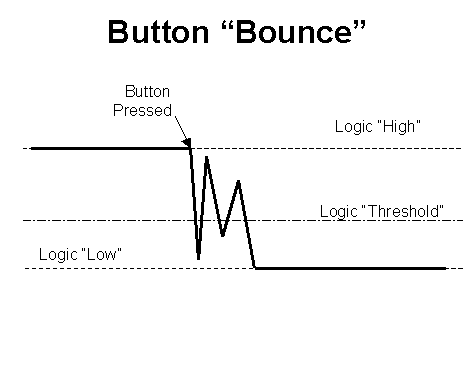
\includegraphics[scale=0.8]{bounce.PNG}
\caption{Button Bounce Waveform}
\footnote{Image courtesy: $https://students.cs.byu.edu/~cs224ta/references/HowTos/HowTo_Interrupts.php$}
\end{figure}
\\
\\
\textbf{Button Bounce:}From the above diagram it is clear that when switch is pressed the signal bounces for a finite amount of time before settling down to its final logic state. This is due to the tendency of any two metal contacts in an electronic device to generate multiple signals as the contacts close or open. The bounce period is ~10 to 20 ms. 
\\
\\
\textbf{Solution: }There are several ways to do button debouncing which includes modifications in both hardware and software. In this lab we will explore software debouncing. In software debouncing too, there are a couple of ways to solve this problem viz. 
\begin{enumerate}
\item  \textbf{Polling the switch plus introducing finite delays:} 
In polling method the controller is busy polling the switch hence it will not be able to perform any other tasks.
\item \textbf{Using interrupts and timers:} If we want to use this time to do other tasks, then we can use interrupts and timers. \\ 
\end{enumerate}
\textbf{Switch debouncing using interrupts and timers:} Check for the status of the switch at finite intervals (say 10 ms). This time interval will be generated using timers. When the 10 ms interval is over the timer should generate an interrupt and the code in the interrupt service routine (ISR) will be executed. In the interrupt service routine, a state machine is implemented. Here the idea is that if the switch pressed for two successive intervals (of 10 ms) then we confirm that the switch is pressed and the next key press is detected only if it is confirmed that switch is released. This will ensure that if a switch press is only detected once. 

A state machine is described below for implementing software debouncing. 
\begin{figure}
\centering
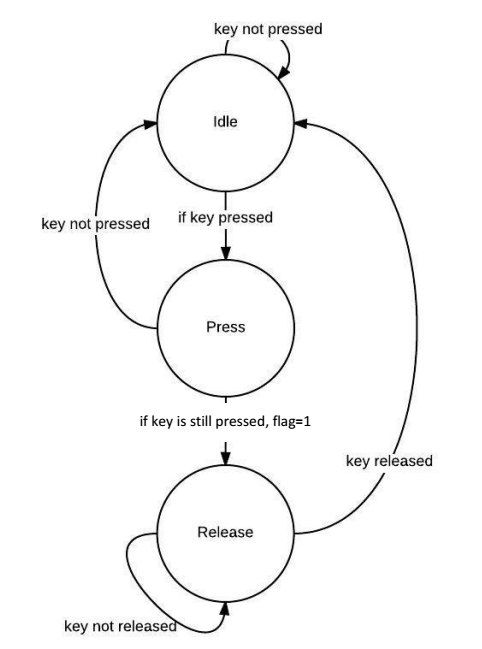
\includegraphics[scale=0.8]{stateChart.png}
\caption{Switch debouncing state diagram}
\label{sm}
\end{figure}
In this state machine there are three states viz. Idle, Press and Release for a switch.
There are two transition paths in each state. Any state transition condition is checked after a fixed interval
of time which is set by a timer (in this case it is 10 ms).
\\
\textbf{Note:} As the bounce period is ~10 ms to 20 ms you can change this time interval based on your experimental
trials. It is possible that different switches have different bounce periods.
\\
\\
\textbf{IDLE} \\
If the key is pressed, enter press state\\
else remain in IDLE state
\\
\\
\textbf{PRESS} \\
If key is still pressed, then enter release state and make flag 1 indicating that key was pressed.\\
else return to idle state (de-bouncing period)
\\
\\
\textbf{RELEASE} \\
If the key is released, then enter an idle state\\
else remain in release state until key is released.


%--------------------------------hardware assembly ---------------
\newpage
\section{Assembly of Hardware}
In this Lab external hardware connections are not required.\\
The PORT pins which will be required are 
\begin{enumerate}
\item PF0 - SW1
\item PF1 - R of RGB
\item PF2 - B of RGB
\item PF3 - G of RGB
\item PF4 - SW2
\end{enumerate}
All these connections are present on the board.


%---------------------------------subsection procedure --------------------------
\section {Procedure}
\subsection{Procedure for Part 1}
\begin{enumerate}
\item Include all the required header files.\\
For using timer and interrupt include :
\begin{lstlisting}
#include "driverlib/interrupt.h"
#include "driverlib/timer.h"
#include "driverlib/pwm.h"
\end{lstlisting}
\item Enable the peripherals (System Clock, PORTF, Timer).
\item Configure PF4 as input and PF1, PF2 and PF3 as output. 
\item Configure the Timer 0 as a 32-bit timer in periodic mode.
\item Calculations :\\
To toggle a GPIO at 10Hz and 50\% Duty Cycle, interrupt is generated at half value of required period.\\
To calculate the number of clock cycles required for 10Hz call \textit{SysCtlClockGet()} and divide it by desired frequency. As interrupt is generated at half value of required frequency, this result is divided by 2. \\
period = (SysCtlClockGet()/10)/2.
\item This calculated period is stored in Timer's Interval Load Register.
\item Enable the interrupt in timer module and NVIC.
\item Enable the Timer.
\item After the calculated period interrupt is generated and a ISR is called.
\item ISR : \\
In ISR check whether the switch is pressed after an interval of 10ms twice.\\
If this condition is satisfied then change the color of RGB.
\end{enumerate}
%------------------------------ part 2 procedure ------------------
\subsection{Procedure for Part 2}
\begin{enumerate}
\item Include all the required header files.\\
For using timer and interrupt include :
\begin{lstlisting}
#include "driverlib/interrupt.h"
#include "driverlib/timer.h"
#include "driverlib/pwm.h"
\end{lstlisting}
\item Declare a global variable \textit{sw2status} to monitor the switch press.
\item Enable the peripherals (System Clock, PORTF, Timer) and unlock PF0.
\item Configure PF0 as input. 
\item Configure the Timer 0 as a 32-bit timer in periodic mode.
\item Calculations :\\
To toggle a GPIO at 10Hz and 50\% Duty Cycle, interrupt is generated at half value of required period.\\
To calculate the number of clock cycles required for 10Hz call \textit{SysCtlClockGet()} and divide it by desired frequency. As interrupt is generated at half value of required frequency, this result is divided by 2. \\
period = (SysCtlClockGet()/10)/2.
\item This calculated period is stored in Timer's Interval Load Register.
\item Enable the interrupt in timer module and NVIC.
\item Enable the Timer.
\item After the calculated period interrupt is generated and a ISR is called.
\item ISR : \\
In ISR check whether the switch is pressed after an interval of 10ms twice.\\
If this condition is satisfied then increment the value of \textit{sw2status}.
\end{enumerate}
%-------------------------- sub section code ---------------------

\section{Code}
\begin{enumerate}
\item \href{https://github.com/eYSIP-2016/eYSIP-2016-Around-the-world-of-Embedded-Systems/blob/origin/master/Solutions/lab2\%20solutions/lab2_1solution.c}{Github link} for solution to Part 1.
\item \href{https://github.com/eYSIP-2016/eYSIP-2016-Around-the-world-of-Embedded-Systems/blob/origin/master/Solutions/lab2\%20solutions/lab2_2solution.c}{Github link} for solution to Part 2.
\end{enumerate}
%---------------------- sub section demo -----------------------
\section{Demonstration Video}

\href{http://10.129.139.139/videos/Lab2.html}{Demo video link} \\
(These videos can be accessed only in IIT Bombay Campus)
 %-------------------------------end of lab 2 ----------------------
 
 
 %--------------------------lab 3 -------------------------------
 \newpage
\chapter{PWM and interfacing Servo Motor}
%---------------------------- objectives subsection-----------------------------
\section{Lab Objectives}
\begin{enumerate}
\item 
Understanding PWM operation in TMS4C123GXL.
\item
Interfacing servo motor with the LaunchPad.
\end{enumerate}


%----------------------sub section pre req---------------------------------------
\section{Pre-requisites}
\begin{enumerate}
\item Lab 1 and Lab 2: Interfacing RGB LED and both the switches.
\item PWM theory
\end{enumerate}


 %------------------sub section - problem statements------------------------------------
\section{Problem Statement}
\textbf{Part 1:} 
Design a RGB LED controller using SW1 and SW2 present in Launchpad board.RGB LED controller has two modes of operation. Auto mode and Manual mode
At initial, when program is loaded controller will be in Auto mode. Combination of SW1 an SW2 has to be pressed to go to Manual mode.When Reset button is pressed, controller will go to Auto mode.
\begin{enumerate}
\item Auto mode
\begin{itemize}
  \item In Auto mode color of the RGB LED follows a pattern in a cycle.
  \item The pattern must follow the color circle as shown in Figure 1.
  \item In Auto mode SW1 will increase the speed of color transition and SW2 will decrease the speed.
\end{itemize}
\begin{figure}
\centerline{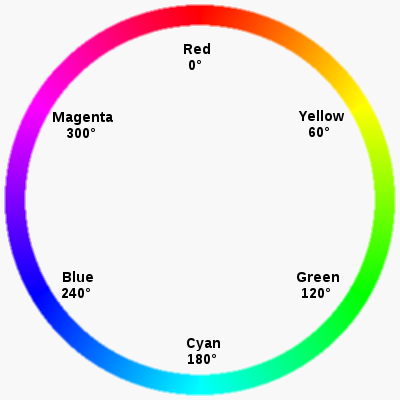
\includegraphics[scale=0.8]{RGB_color_circle.png}}
\footnote{Image Courtesy: https://en.wikibooks.org/wiki/File:RGB\_color\_circle.png accessed on 05/06/2016}
\caption{RGB Color Wheel}
\end{figure}

\item Manual mode
\begin{itemize}
\item In Manual mode, user must be able to select any one of the color from the color circle. For this
intensity of any of the 3 LEDs must be controlled independently.
\item Mode 1 (Red LED control) - When SW2 is pressed continuously(long press) and SW1 is pressed
once controller goes to Manual Mode 1. In this mode, intensity of Red LED can be controlled using
SW1 and SW2.
\item Mode 2 (Blue LED control) - When SW2 is pressed continuously(long press) and SW1 is pressed
twice controller goes to Manual Mode 2. In this mode, intensity of Blue LED can be controlled using
SW1 and SW2.
\item Mode 3 (Green LED control) - When SW1 and SW2 are pressed continuously controller goes to
Manual Mode 3. In this mode, intensity of Green LED can be controlled using SW1 and SW2.
\end{itemize}

\end{enumerate}
\textbf{Part 2:}
Interfacing a servo motor and controlling it using a switch.
\begin{enumerate}
\item When switch 1 is pressed the motor should rotate by ten degrees clockwise.
\item When switch 2 is pressed the motor should rotate by ten degrees anti-clockwise.
\item While doing the above two actions check for limits of the servo motor. It should no move beyond the operating range.
\item Use the switch debouncing method for interfacing the switch.
\end{enumerate}




 %-------sub section Relevant theory---------------------------
 
\section {Relevant Theory}
\begin{enumerate}
\item  Refer \textit {TM4C123G\_LaunchPad\_Workshop\_Workbook} available on course web page.Texas.Refer Chapter-15. 
\end{enumerate}

%--------------------------------hardware assembly ---------------
\section{Assembly of Hardware}
For part 1 external hardware connections are not required.\\
For part 2 connect the pin PD0 as PWM input to Servo Motor.\\
\begin{enumerate}
\item PF0 - SW1
\item PF1 - R of RGB
\item PF2 - B of RGB
\item PF3 - G of RGB
\item PF4 - SW2
\item PD0 - PWM Output
\end{enumerate}

%-----------------------------Procedure -------------------
\section{Procedure}
\begin{enumerate}
\item Include all the header files. Ensure that the following header files are present.\\
 include "driverlib/pwm.h"\\
 include "driverlib/timer.h"\\
 include "driverlib/interrupt.h"
 \item Configure the PORT Pins as PWM outputs and configure the PWM generator depending on the PWM pin used.
 \item  Enable the PWM output state.
 \item  Enable the PWM generator. 
\item For Part 1 - \\Depending on the color wheel switch on the respective LEDs. Do not turn off the LED completely by assigning 0 value to it as it causes it to turn ON with a high intensity. Instead assign a minimum non-zero value to it so as to reduce the intensity.   

\item For Part 2 - \\Calculate the value of PWM period. \\
eg. In this code PWM base frequency is taken as 50Hz. The total period of Servo Motor is 1/50 = 20 ms. \\ 
The oscillator frequency is 40MHz. This value is divided by 64. The answer is further divided by the PWM base frequency(50Hz).
Thus Period=12500. 
\end{enumerate}

%-------------------------- sub section code ---------------------
\section{Code}
\begin{enumerate}
\item \href{https://github.com/eYSIP-2016/eYSIP-2016-Around-the-world-of-Embedded-Systems/blob/origin/master/Solutions/lab3\%20solutions/lab3_solution1.c}{Github link} for solution to Part 1.
\item \href{https://github.com/eYSIP-2016/eYSIP-2016-Around-the-world-of-Embedded-Systems/blob/origin/master/Solutions/lab3\%20solutions/lab3_solution2.c}{Github link} for solution to Part 2.
\end{enumerate}
%---------------------- sub section demo -----------------------
\section{Demonstration Video}
\href{: http://10.129.139.139/videos/Lab3.html}{Demo video link}\\
(These videos can be accessed only in IIT Bombay Campus)
%----------------------end of lab 3 -----------------------


%-------------------lab 4 ------------------------------

\chapter{ADC and Serial Communication}
%--------------- objective ----------------------------
\section{Lab Objective}
Use of the analog to digital conversion (ADC) peripheral and Universal Asynchronous Receiver/Transmitter (UART) on the TM4C123GH6PM.


%------------ pre requisites --------------
\section{Pre-requisite}
Go through the documents in relevant theory section.


%------------------ problem statement ----------------
\section{Problem Statement}
\begin{enumerate}
\item 
Using the inbuilt ADC to interface a joystick with Tiva Board. The analog values read from the joystick have to be converted to digital and displayed on the watch window of the CCS IDE.For information about the joystick pinout refer to the figure below:
\begin{figure}
\centering
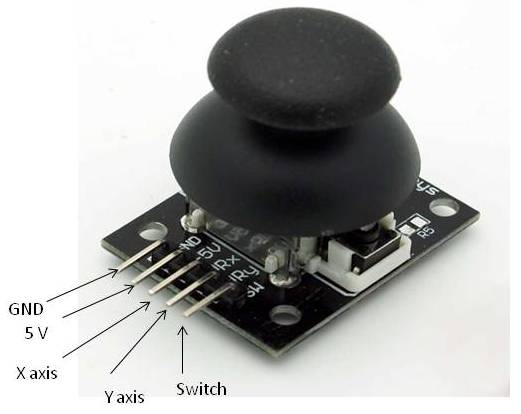
\includegraphics[scale=0.5]{joystick_pinout.jpg}
\caption{Joystick Pinout}
\end{figure}
\item
The inbuilt UART is used to communicate the digital values (i.e. both the X axis and the Y axis) to the computer.A terminal emulation software like Serial Terminal or Real Term can be used to view the data being sent by the Tiva Board to computer.
\newline
\hspace{10mm} \textit{The data sent should have the following syntax :}
\newline
\hspace{10mm}\textit{"X: Digital equivalent of the read value"}
\newline
\hspace{10mm}\textit{"Y: Digital equivalent of the read value"}
\item
Once you complete the above mentioned problem statements, you have to depict the values received in a graphical representation. In short, create a GUI which tracks the real time movements of the joystick.
\newline
Refer to the Figure 1, the circle marker should move to the left if the joystick button is tilted towards left and right if tilted towards right. The marker should remain at the centre when joystick is stationary.
\end{enumerate}
\begin{figure}
\centering
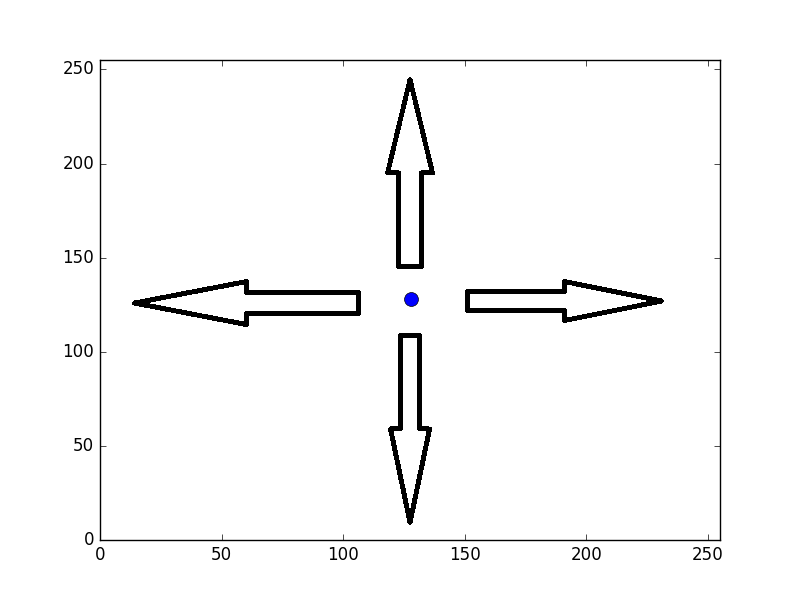
\includegraphics[scale=0.4]{joystickgui.png}
\caption{Joystick Graphical interface}
\end{figure}


%------------------ Relevant theory -------------------
\section {Relevant Theory}
Some general terms related to ADC.
\footnote{EE712 Embedded Systems, presentation from WEL Lab}
\begin{enumerate}
\item \textbf{Sample Sequencer}
The sampling control and data capture is handled by the sample sequencers.
The sample sequencers can be assumed to be a module with memory, which can sample different analog sources with a single trigger event without processor intervention.
All of the sequencers are identical in implementation except for the number of samples that can be captured and the depth of the FIFO.
\item \textbf{Trigger Source}
ADC can be triggered by various sources like processor, external GPIO, PWM, internal comparators, timer etc.
\item \textbf{Relative Priority}
There are 4 sample sequencers. Hence, we need to specify the relative priority of a sequencer in case we are using multiple sample sequencers.
\item \textbf{GPIO Pins}
There are 12 analog input channels shared by two Analog-to-Digital Converter modules. Certain GPIO pins can act as input channels for these ADC modules. For information about these pins, refer to section 12, pages 799 - 801 of \textit{Datasheet} . Use GPIOPinTypeADC() function to configure these pins.Refer to page 266 of \textit{Peripheral Driver Library} for detailed description of this function.
\end{enumerate}
Detailed description of theory and code examples are available in the following links:
\begin{enumerate}
\item Refer \textit{TM4C123G\_LaunchPad\_Workshop\_Workbook} chapter 5 for ADC12.
\item Refer \textit{TM4C123G\_LaunchPad\_Workshop\_Workbook} chapter 7 for UART.
\end{enumerate}

\textbf{Joystick Graphical User Interface:}
\newline
You can use any open source programming language to build your GUI. Below, we have listed down some pointers to assist you, if you choose python
\begin{enumerate}
\item The first step is to read serial data coming on your COM port. Use pyserial library to do so.
\item If you notice carefully, GUI only requires five distinct values, you can avoid sending other values in your embedded C code. Also the rate at which Joystick data is sampled can also be reduced.
\item
Once you start receiving your required data, you can use matplotlib and drawnow library to get a real time Graphical representation. There are several other libraries that can be used to get a real time representation, you are free to use any of them. 
\end{enumerate}


%-------------- Procedure -------------------
\section {Procedure}

\subsection{ For ADC and UART code :}
\begin{enumerate}
\item Include "adc.h" and "uart.h" header files.
\item Enable ADC0 and ADC1 peripherals. Enable and configure the UART pins. Set the required Baud rate.
\item Wait till ADC conversion is complete. Take average of the data obtained. This is then converted according to requirements. 
\item Send the ASCII value of this data to Computer using UART.
\end{enumerate}
\subsection{To create GUI in Python}
\begin{enumerate}
\item Import serial library, matplotlib, numpy.
\item Read the serial data.
\item Enable the interactive plot using plt.ion() function.
\item Split the received co-ordinates at comma and convert it into float.
\item Plot these co-ordinates using "drawnow()" function.    
\end{enumerate}


%-------------------- Code -------------------
\section{Code}
\begin{enumerate}
\item \href{https://github.com/eYSIP-2016/eYSIP-2016-Around-the-world-of-Embedded-Systems/blob/origin/master/Solutions/lab4\%20solutions/lab4_solution.c}{Github link} to use ADC and UART.
\item \href{https://github.com/eYSIP-2016/eYSIP-2016-Around-the-world-of-Embedded-Systems/blob/origin/master/Solutions/lab4\%20solutions/gui.py}{Github link} for GUI in Python.
\end{enumerate}


%---------------------- Demo --------------------
\section{Demonstration Video} 
\href{http://10.129.139.139/videos/Lab4.html}{Demo video link.}\\
(These videos can be accessed only in IIT Bombay Campus)
%--------------------- lab 4 end ---------------------

%---------------lab 5 ----------------------------------
\chapter{Temperature Sensor(LM35) and LCD}

%lab Objective
\section{Lab Objective}
Interfacing a 16x2 LCD with the TIVA board and LM35 temperature sensor.


%--------------- pre req------------------------
\section{Pre-requisite}
\begin{enumerate}
\item 
Lab 4 : ADC and UART
\item Working of 16x2 LCD and interfacing it in 4 bit mode.
\end{enumerate}


%----------------- Problem Statement------------------------------------
\section{Problem Statement}

\begin{enumerate}
\item 
Interface a 16x2 LCD in 4 bit mode with the board. There is an onboard temperature sensor, display the temperature sensed by this sensor on the LCD; use the internal ADC to convert analog readings to digital ones.
\item
Next, interface an external LM35 temperature sensor with the board and display the temperature on the LCD. Use the switch "sw1" to switch between internal and external temperature readings. The display should show external sensor readings by default and switch to internal when"sw1" is pressed once, on the next press the display should return to default (show external temperature readings). Figure 2 below will clear things out.
\end{enumerate}

Follow the display format as shown in the figure 1 below:
\begin{figure}
\centering
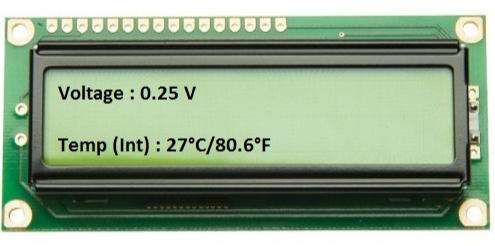
\includegraphics[scale=0.6]{lcd.PNG}
\caption{LCD Display Format}
\centering
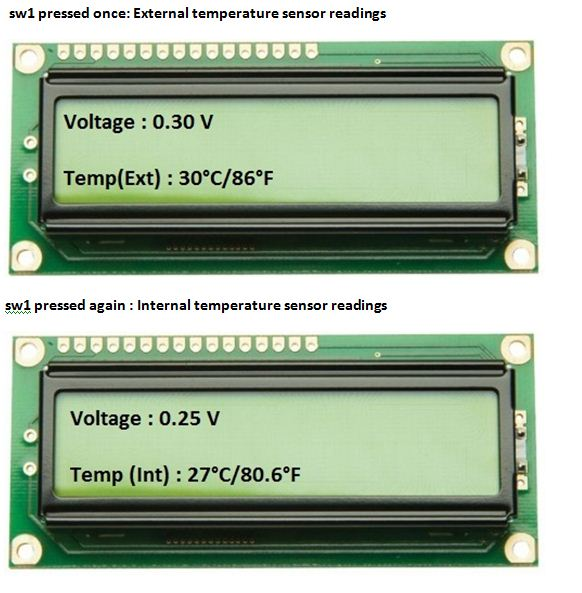
\includegraphics[scale=0.5]{flow.JPG}
\caption{Alternating sensor display values}
\end{figure}



%---------------------Relevant Theory--------------------------------
\newpage
\section {Relevant Theory}
\begin{enumerate}
\item This lab will use LM35 temperature sensor, you can refer to its datasheet from the following link:\href{http://www.ti.com/product/LM35/datasheet}{\textbf{Datasheet}}.
\item 
LCD has to be used in 4 bit mode. Go through the commands required to interface LCD in 4 bit mode.
\item 
The problem statement requires you display decimal values upto two places on the LCD. You can shift the values to the left by appropriate places and then use the ascii value of "." to display decimal values.  
\item 
Please follow the timings given in the LCD data sheet during initialization. 
\end{enumerate}


%------------------------ procedure ---------------------------------
\section {Procedure}

\subsection{For using  LCD in 4 bit mode :}
\begin{enumerate}
\item First initialize LCD in 4 bit mode
\item Give commands for clear screen,display on and cursor location
\item Command mode:
 In command mode RS=0 and RW=0. \\
 Send higher 4 bit.\\
After sending data to the port;give a enable pulse.\\
 Send lower 4 bit.\\
 After sending data to the port;give a enable pulse.\\
 Give delay of microsecond at end.
\item Write mode:
In write mode RS=1 and RW=0\\
Send higher 4 bit\\ 
After sending data to the PORT generate high to low enable pulse \\
Send lower 4 bit\\ 
After sending data to the PORT generate a high to low enable pulse \\
Give delay of microsecond at end\\
\end{enumerate}
\newpage
\subsection{For external temperature conversion:}
\begin{enumerate}
\item Configure ADC1 chip.
\item Set ch1 to get analog data.
\item Enable ADC1. 
\item Wait until interrupt has occurred,
\item Store the data in the variable and convert it into Celsius by dividing it with 12.41.
\item Convert the stored data into character and store it in array.
\item Send the character array to LCD screen.
\end{enumerate}

\subsection{For internal temperature}
\begin{enumerate}
\item Configure ADC0 chip.
\item Set the temperature given on chip.
\item Enable ADC0.
\item Wait until interrupt has occurred.
\item Store the data in variable and convert data into Celsius.
\item Convert the stored data into character and store it in array.
\item Send the character array to LCD screen.
\end{enumerate}



%-------------------------------- Code ----------------------
\section{Code}
\href{https://github.com/eYSIP-2016/eYSIP-2016-Around-the-world-of-Embedded-Systems/blob/origin/master/Solutions/lab5solution/lab5_solution.c}{Github link} of solution.




%---------------------------- Demo -------------------------
\section {Demonstration}
\begin{enumerate}
\item \href{ http://10.129.139.139/videos/Interfacing_LCD_TIVA_Launchpad.html}{LCD Interfacing Tutorial}
\item \href{http://10.129.139.139/videos/Lab5.html}{Demo video link}
\end{enumerate}
(These videos can be accessed only in IIT Bombay Campus)
\newpage






%---------------------------- end of labs -----------------

%------------------- project 1 -------- line following robot ---------

\newpage
\chapter{Project 1:Line follower robot}
\section*{Abstract:}

Project is about making line following robot using TIVA board.For devolping this robot,the modules used are ADC,PWM and GPIO.Using ADC pin,conversion of analog value of white line sensor to digital value.PWM pin is used for controlling the speed of motor and GPIO pin can be used for moving motor clockwise and anti-clockwise.One additional module of EEPROM is also included.EEPROM is used to store the threshold value of the sensor so if robot is again turn on, the robot  will regain it's value from EEPROM.Thus,no need to calibrate sensor every time and also it can perform auto-calibration of sensor.In this function ,the threshold value of black and white line are stored in EEPROM.On pressing of sw1 switch it goes to calibration mode and does the calibration by storing threshold value in EEPROM.Thus,every time calibration is not needed and as the value is stored in EEPROM,it can be regained after restarting the robot.Thus,every time we don't need to calibrate as the value is stored in EEPROM.   

 %------------------sub section objective ------------------------------------------
\section*{Completion Status:}
It follows white line and goes to auto mode and stores value in eeprom.
\section{Software used}
\begin{enumerate}
  \item Code Composer Studio\\  
  Version 6.1.2 \\
  \href{http://processors.wiki.ti.com/index.php/Download_CCS}{CCS Download Link}\\
  \href{http://processors.wiki.ti.com/index.php/GSG:CCSv6_installation}{CCS Installation steps}
  \item TivaWare\_C\_Series-2.1.2.111\\
  \href{http://www.ti.com/tool/sw-tm4c}{Download Link}
\end{enumerate}
\section{Hardware Parts:}
\begin{enumerate}
\item Two dc motor
\item White line sensor
\item Motor driver ic
\item Power Bank
\item Two wheel
\end{enumerate}

\section{Pin Diagram:}
\begin{enumerate}
\item

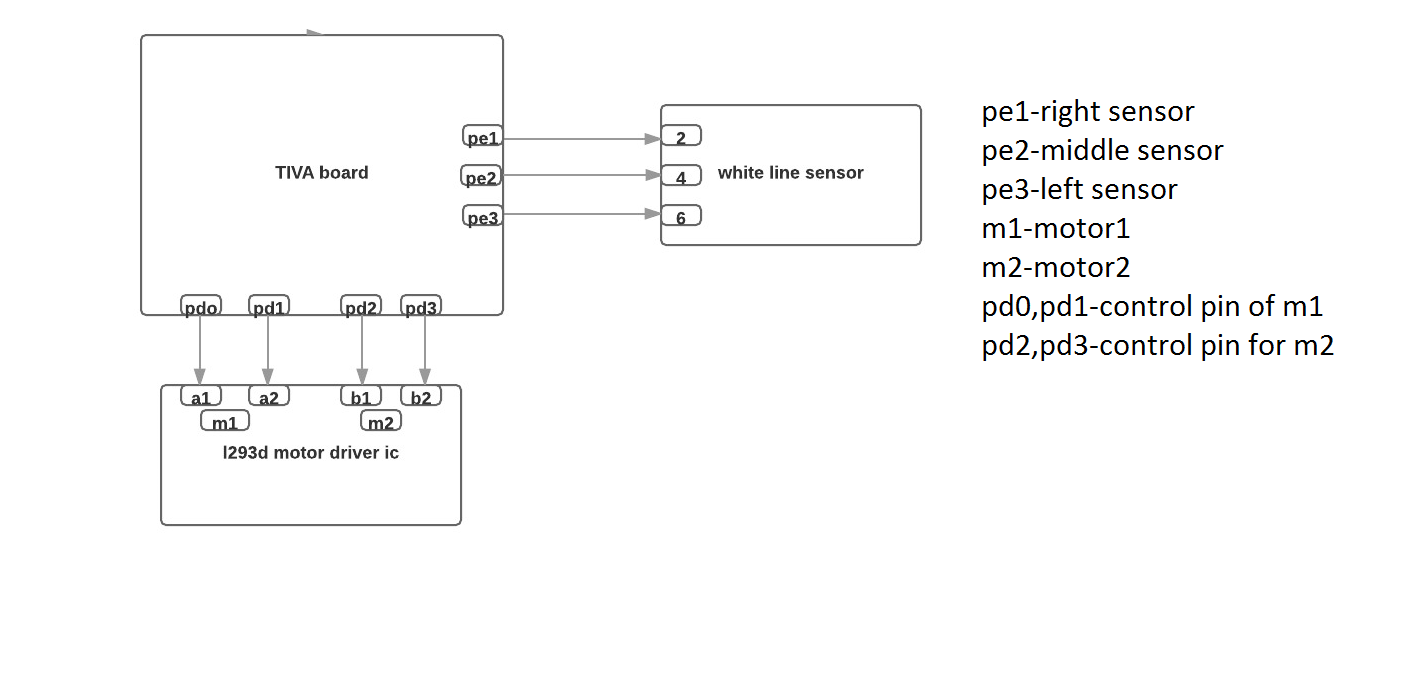
\includegraphics[width=400 px]{pin.png}

\end{enumerate}

\section{Assembly of hardware:}
\begin{enumerate}
\item Hardware required for assembly.

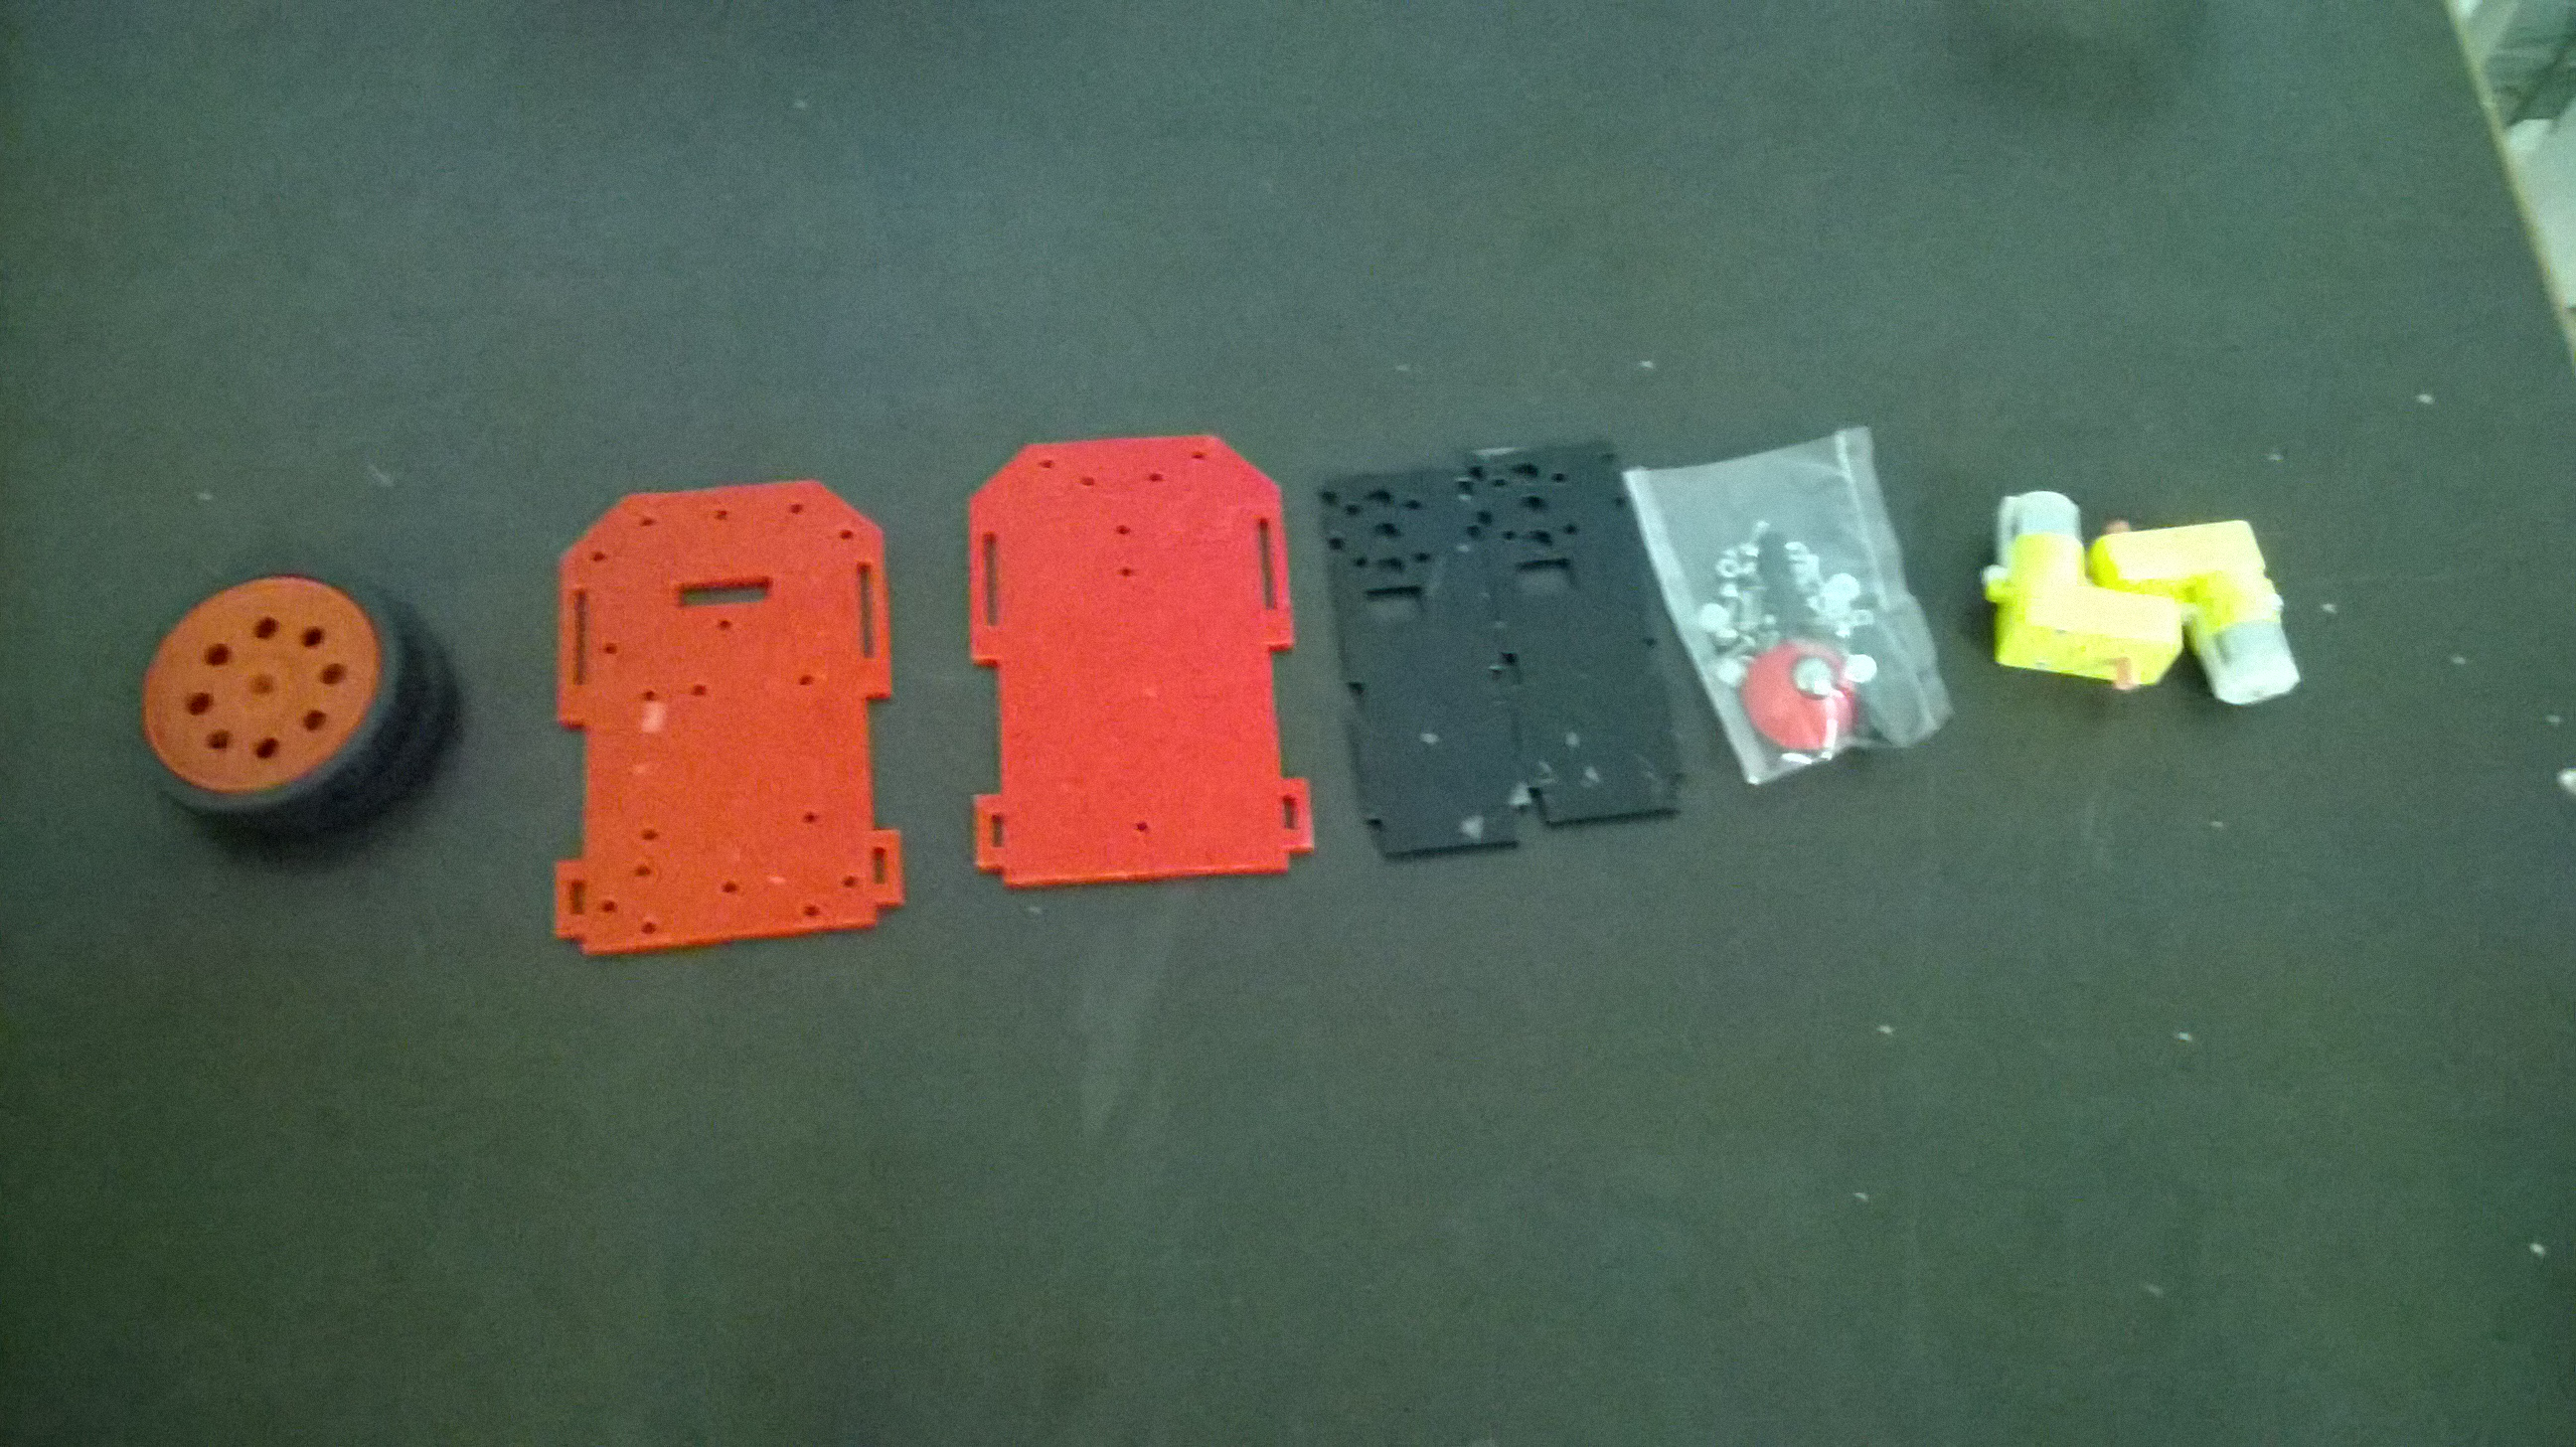
\includegraphics[width=400 px]{hardware.jpg}

\item Assemble the body of robot.

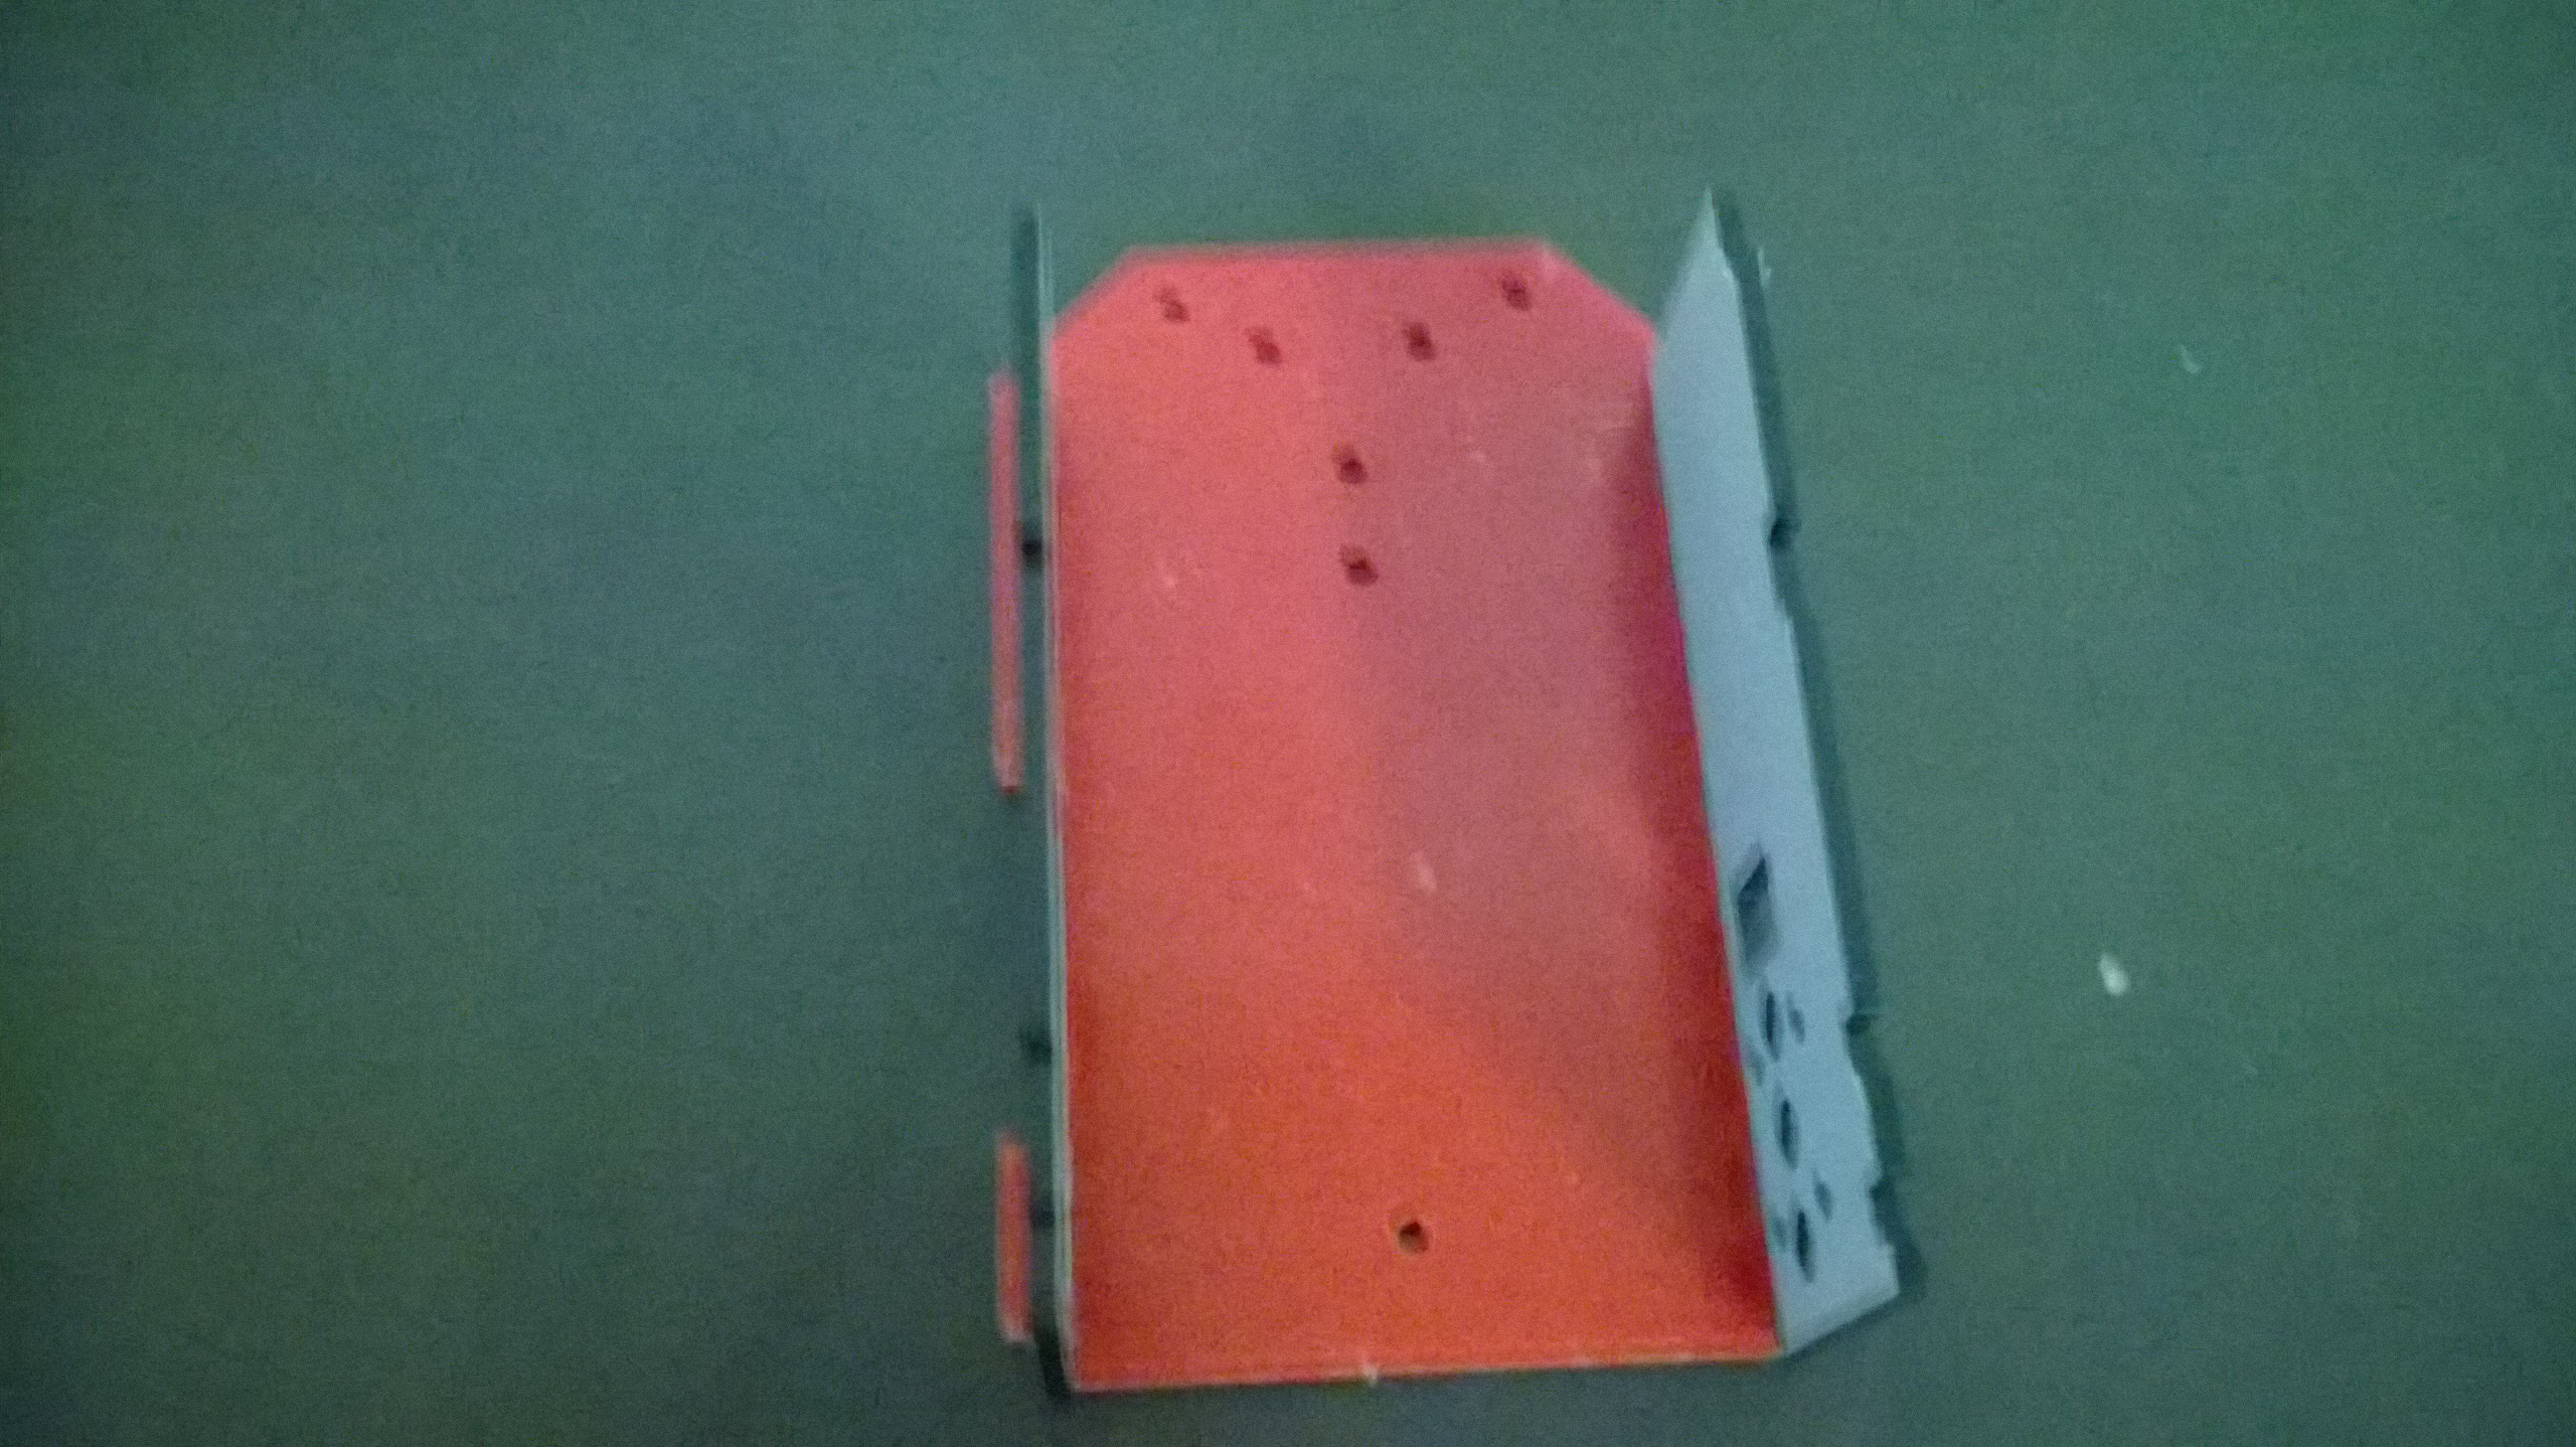
\includegraphics[width=400 px]{chassey.jpg}

\item Attaching the dc motor and wheel through screw.

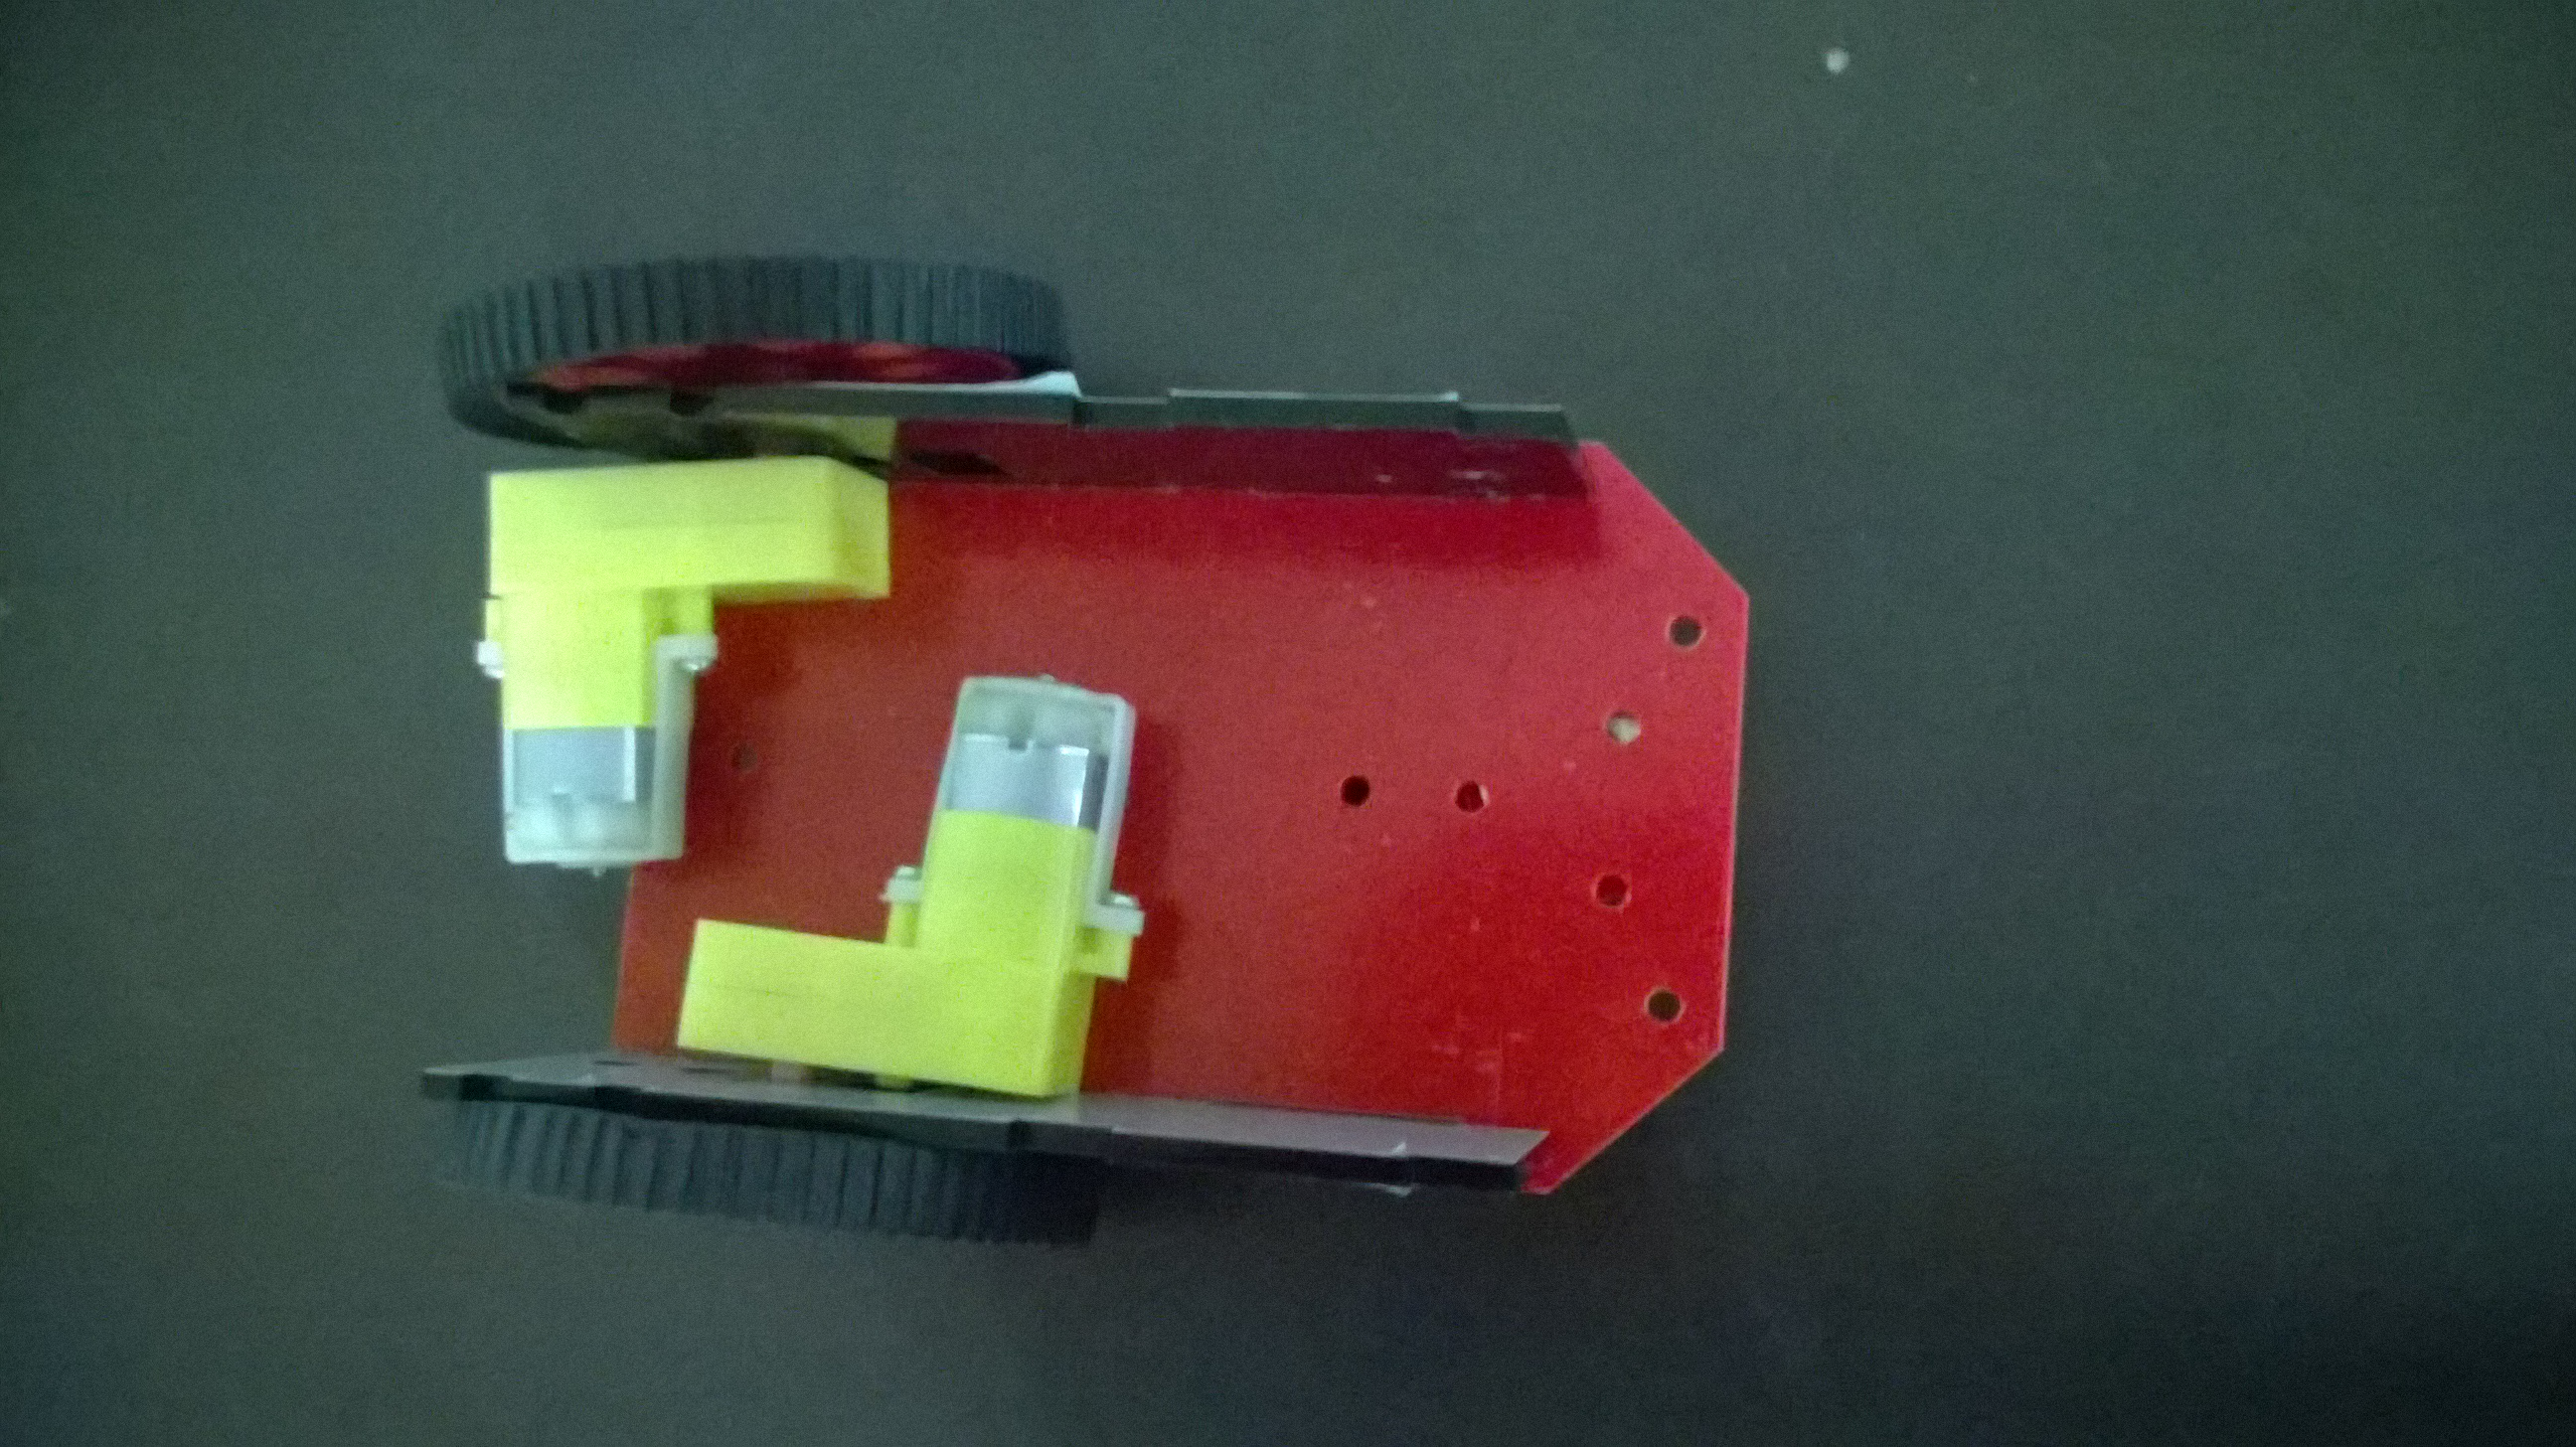
\includegraphics[width=400 px]{attaching_dc_motor.jpg}

\item Increase the height of top through the support as shown in figure and also attach the white line sensor.AS, on increasing the height of robot,the body will remain loss,so apply glue gun so chassey of robot becames stable.

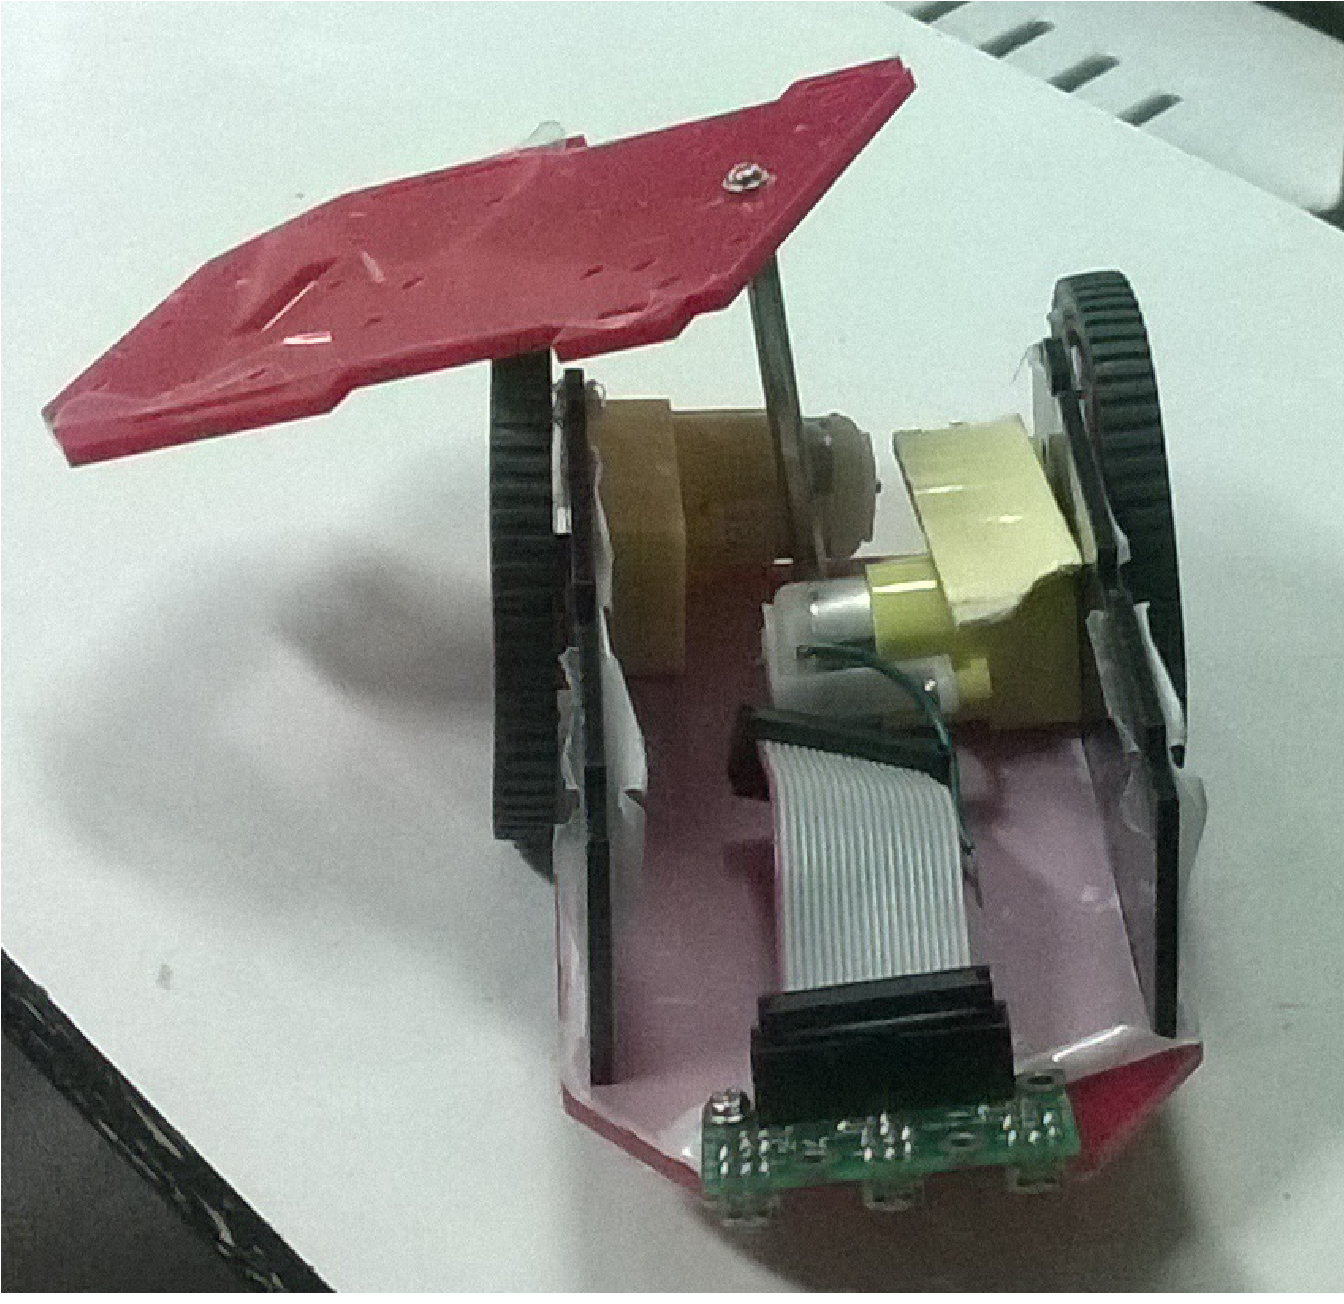
\includegraphics[width=400 px]{img6.png}



\item Now on genral pcb make the connection as shown in figure.

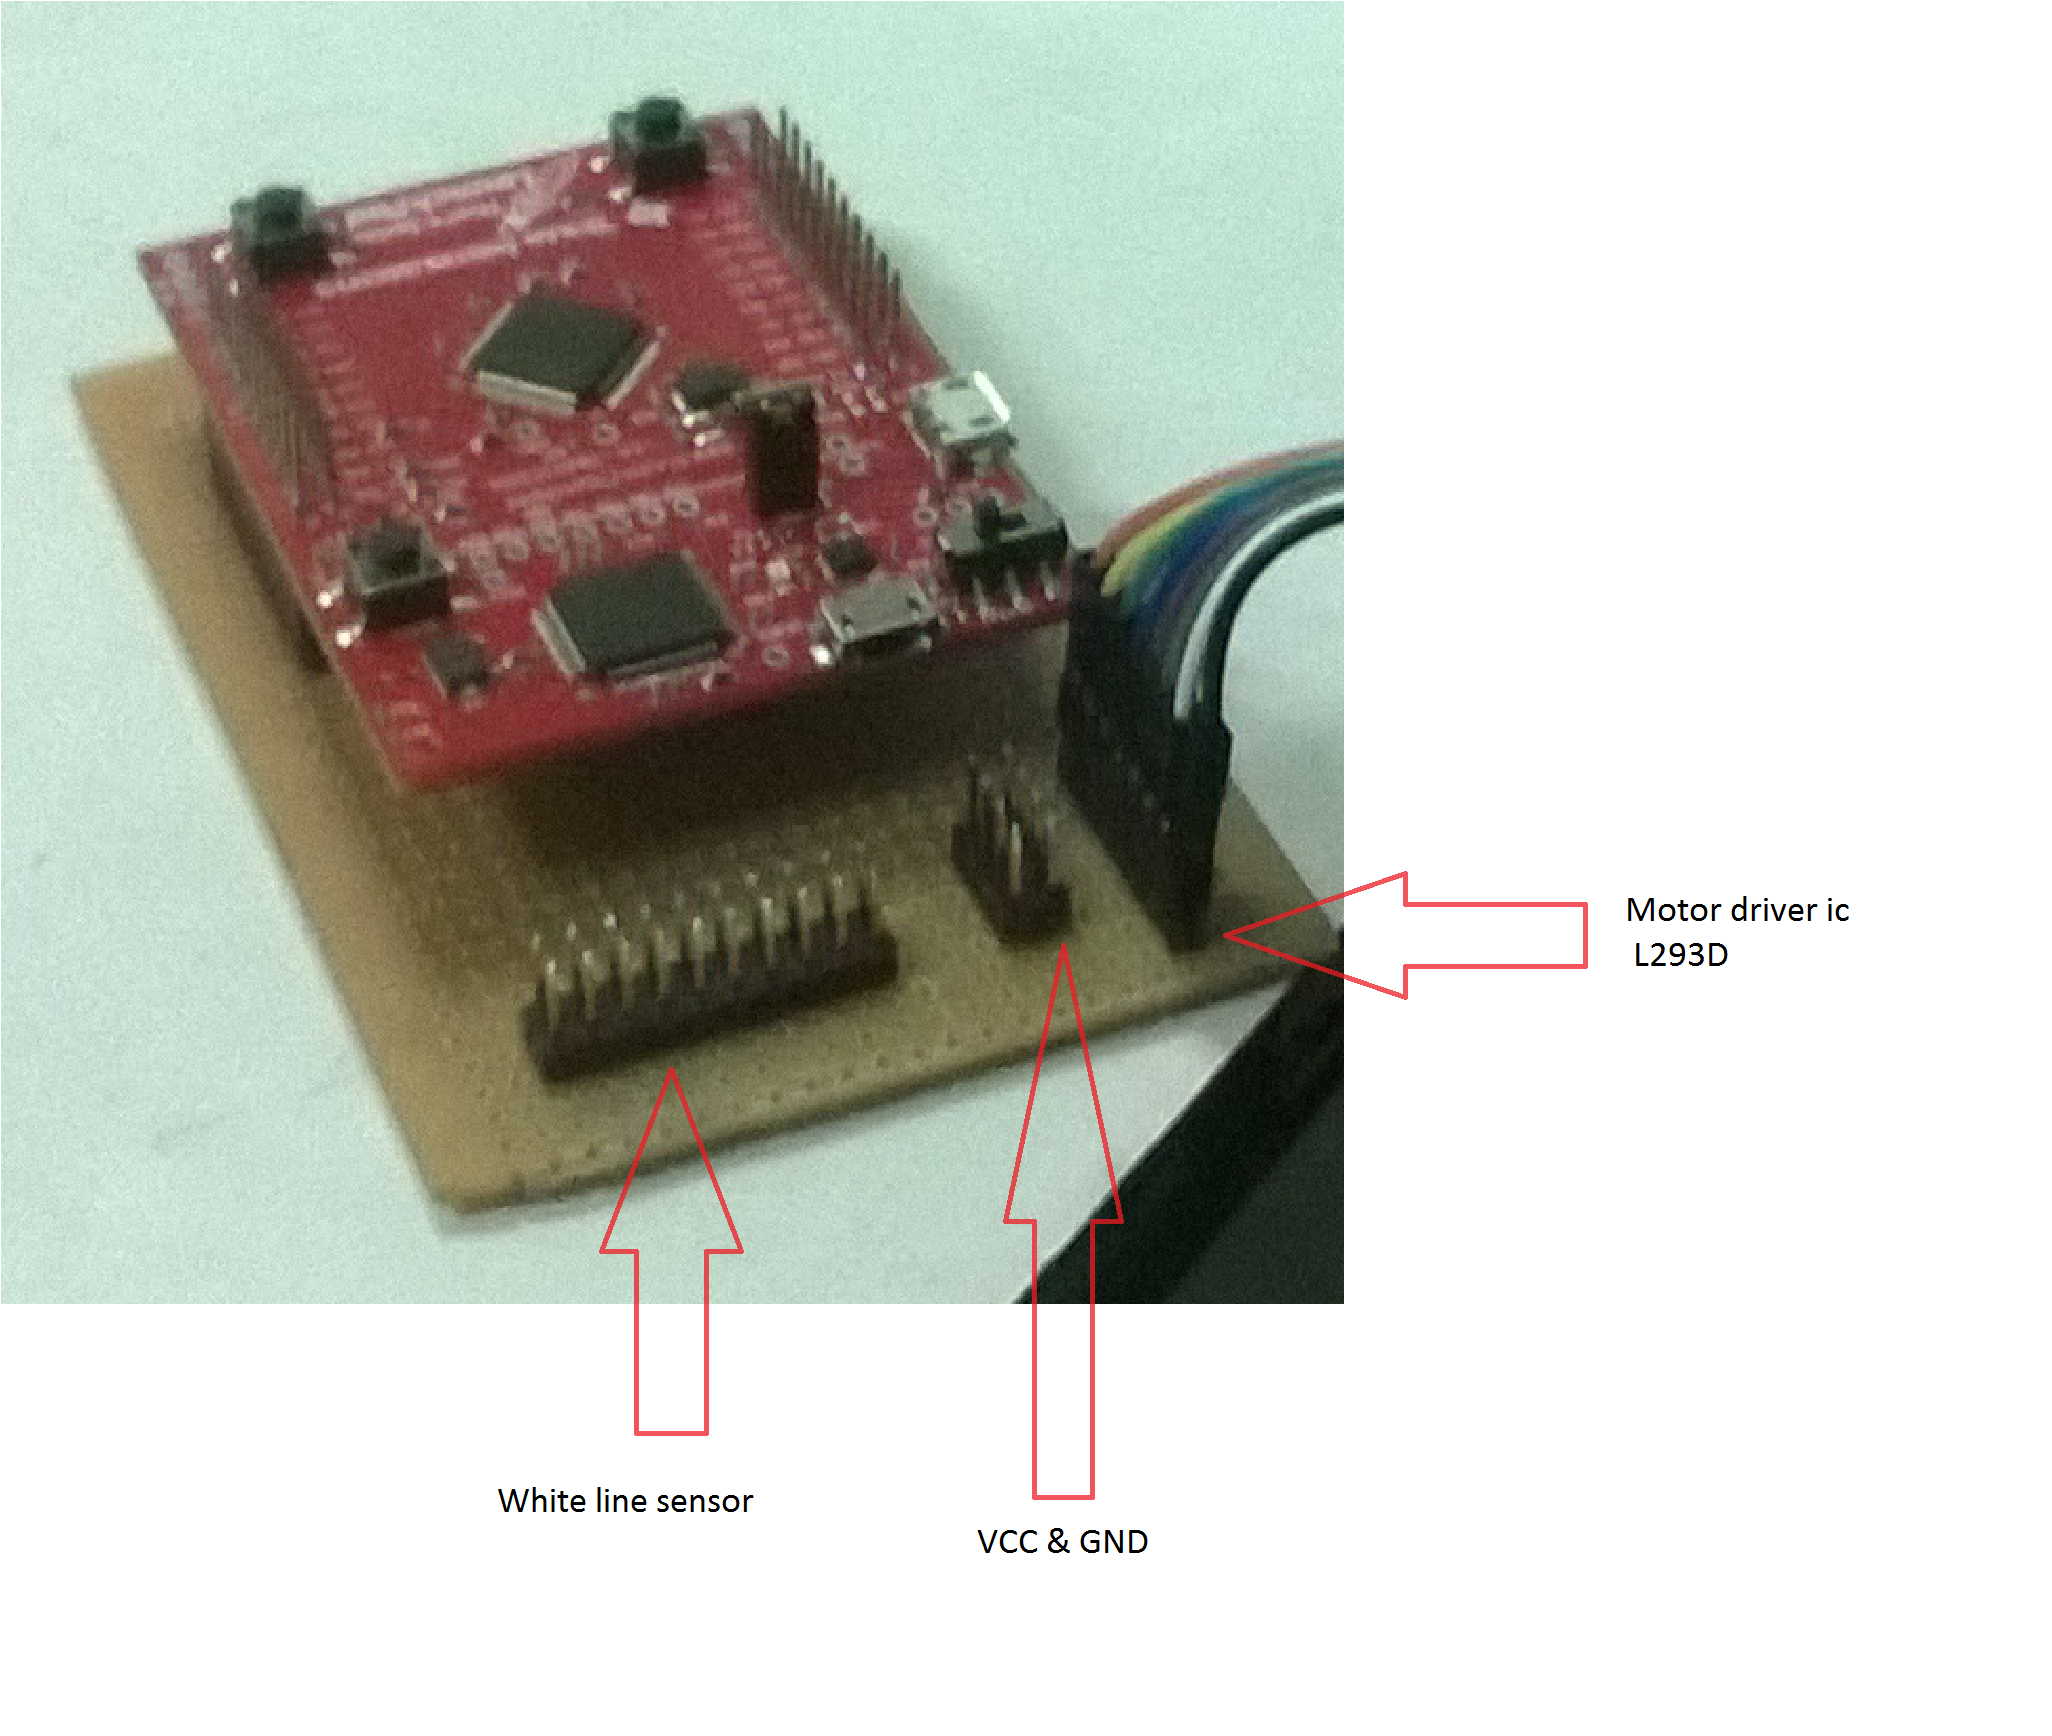
\includegraphics[width=300 px]{pcb.png}

\item Connect the motor driver ic, white line sensor with tiva. Now,load the program and on the debug mode.Add variable x,y,z as watch expression and observe the value on computer.This procedure enables to varify if robot is working properly or not. 

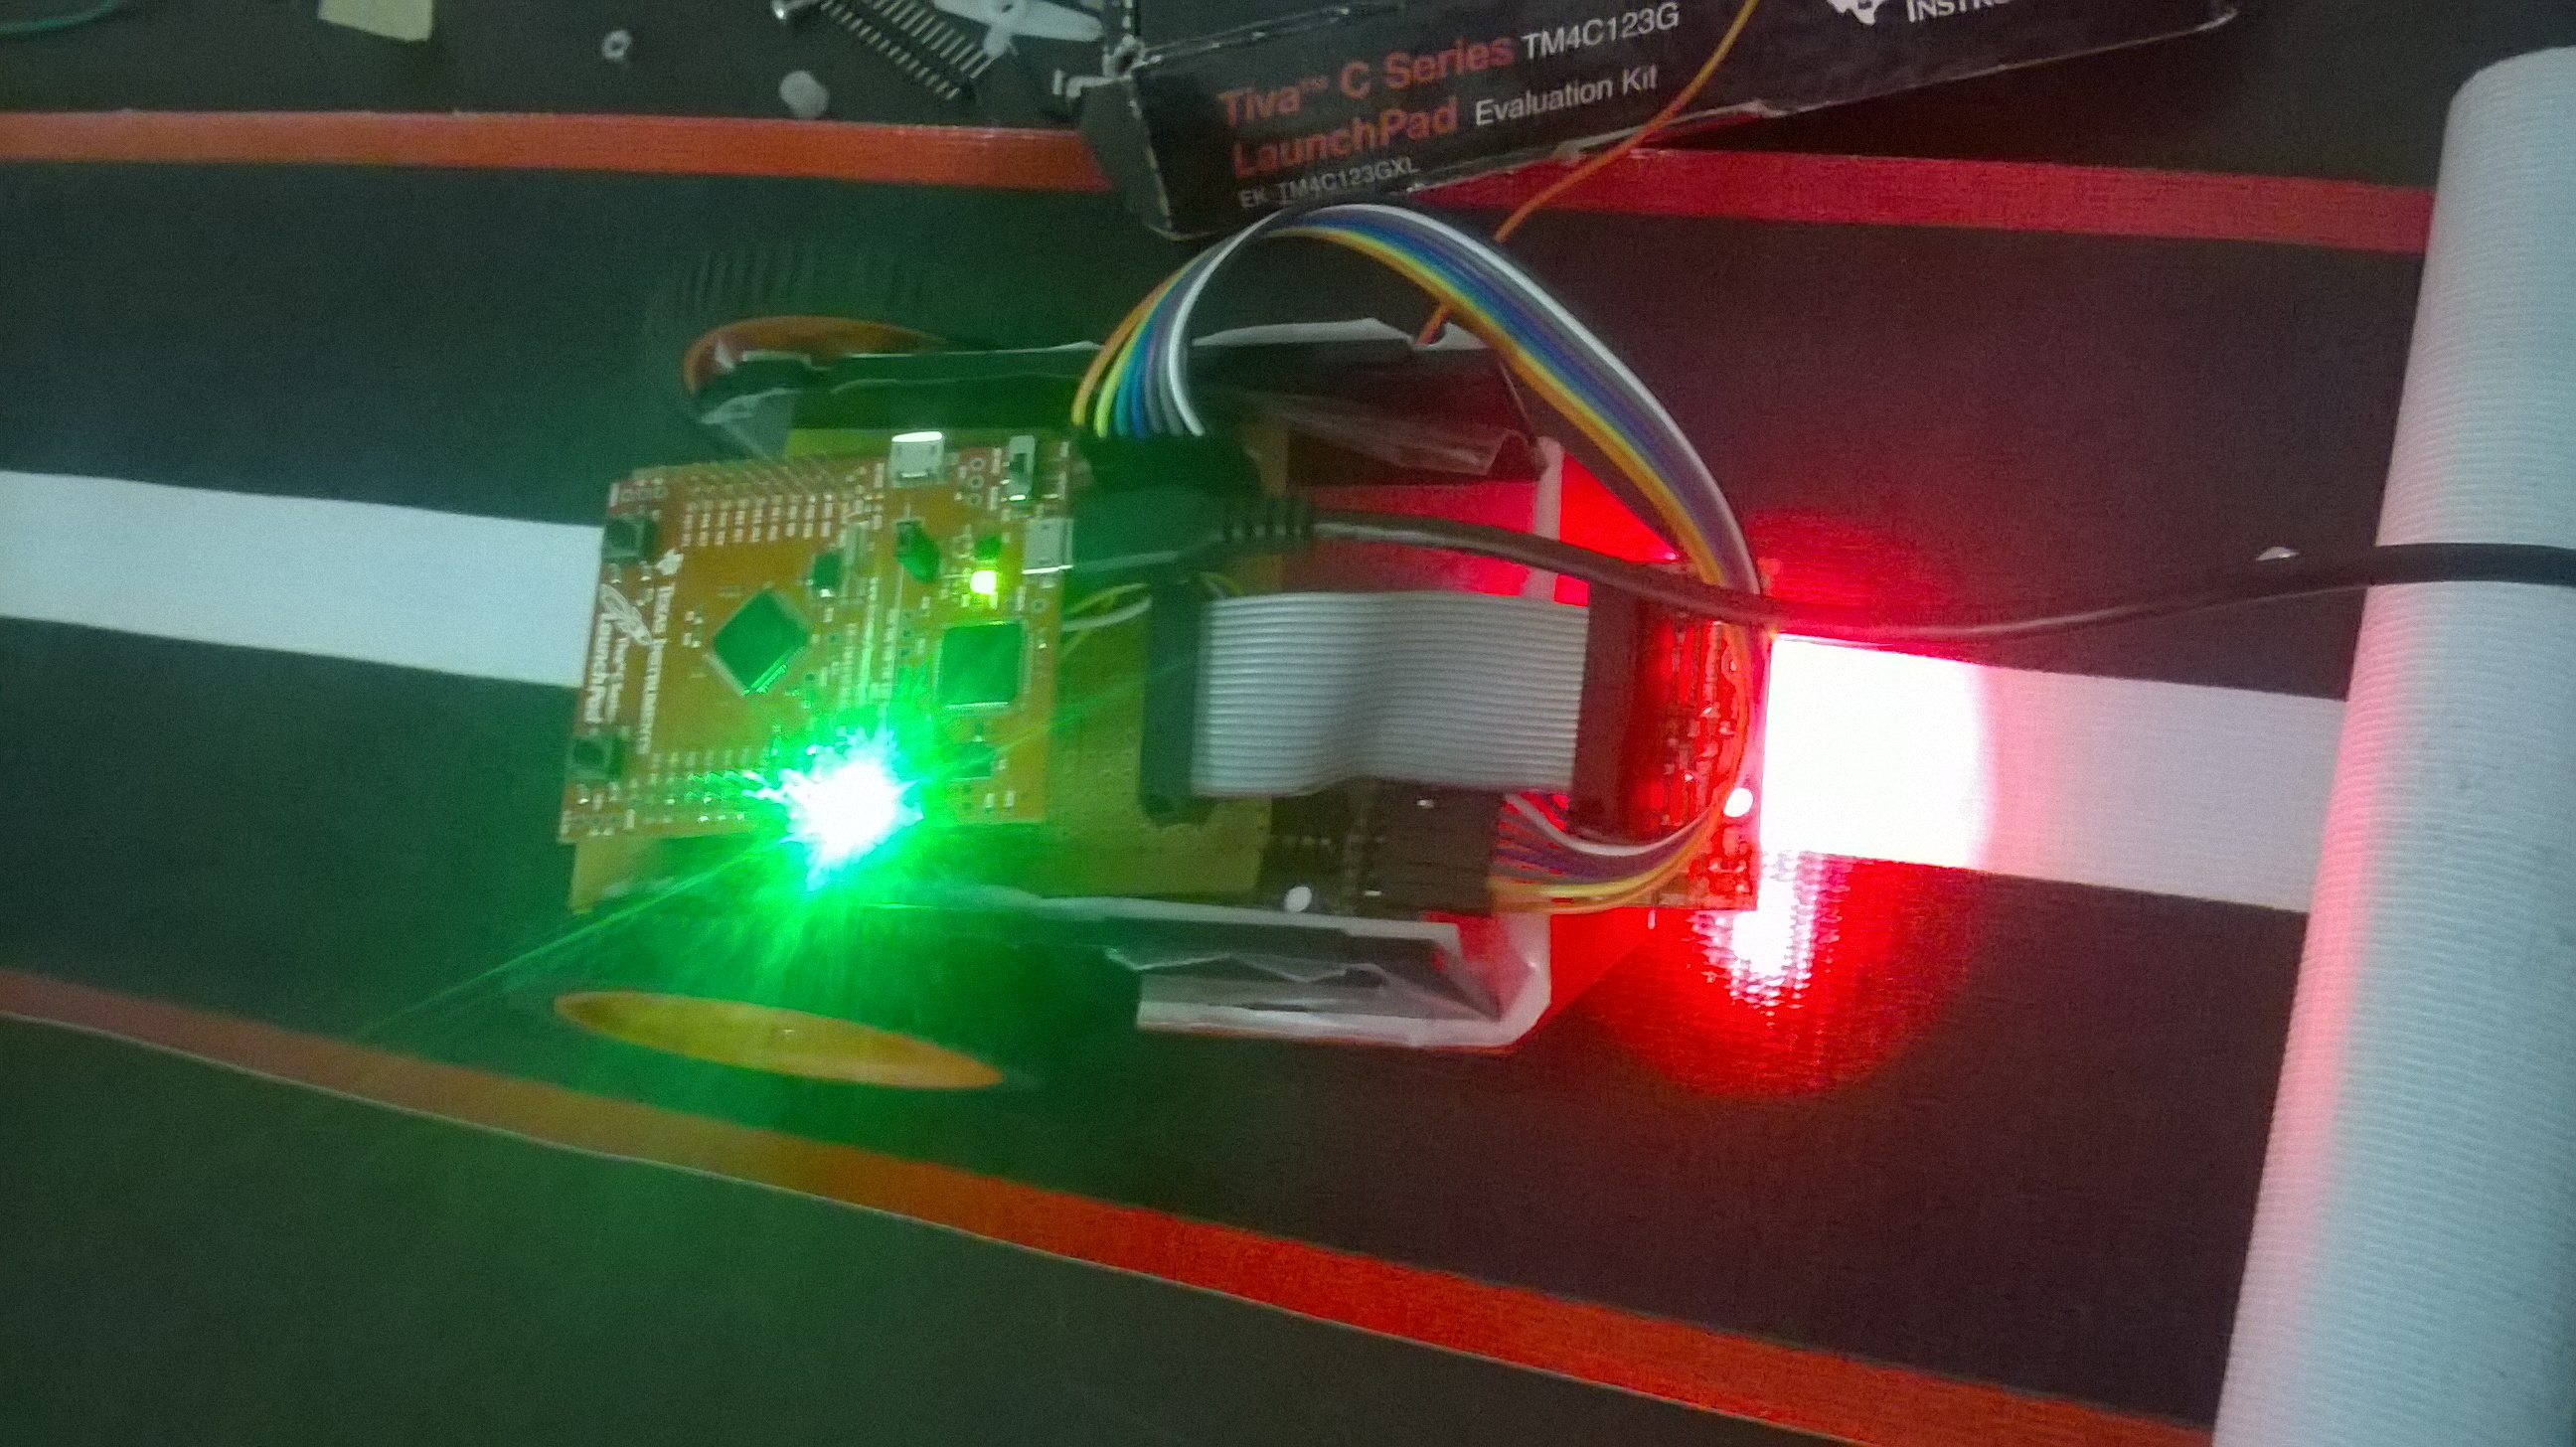
\includegraphics[width=400 px]{calibration.jpg}

\item Attach the power bank and also connect 9 volt battery to motor driver ic.Additional 9 volt battery is connected because power from TIVA board was not adequate to run DC motor. final robot will look as shown in figure.

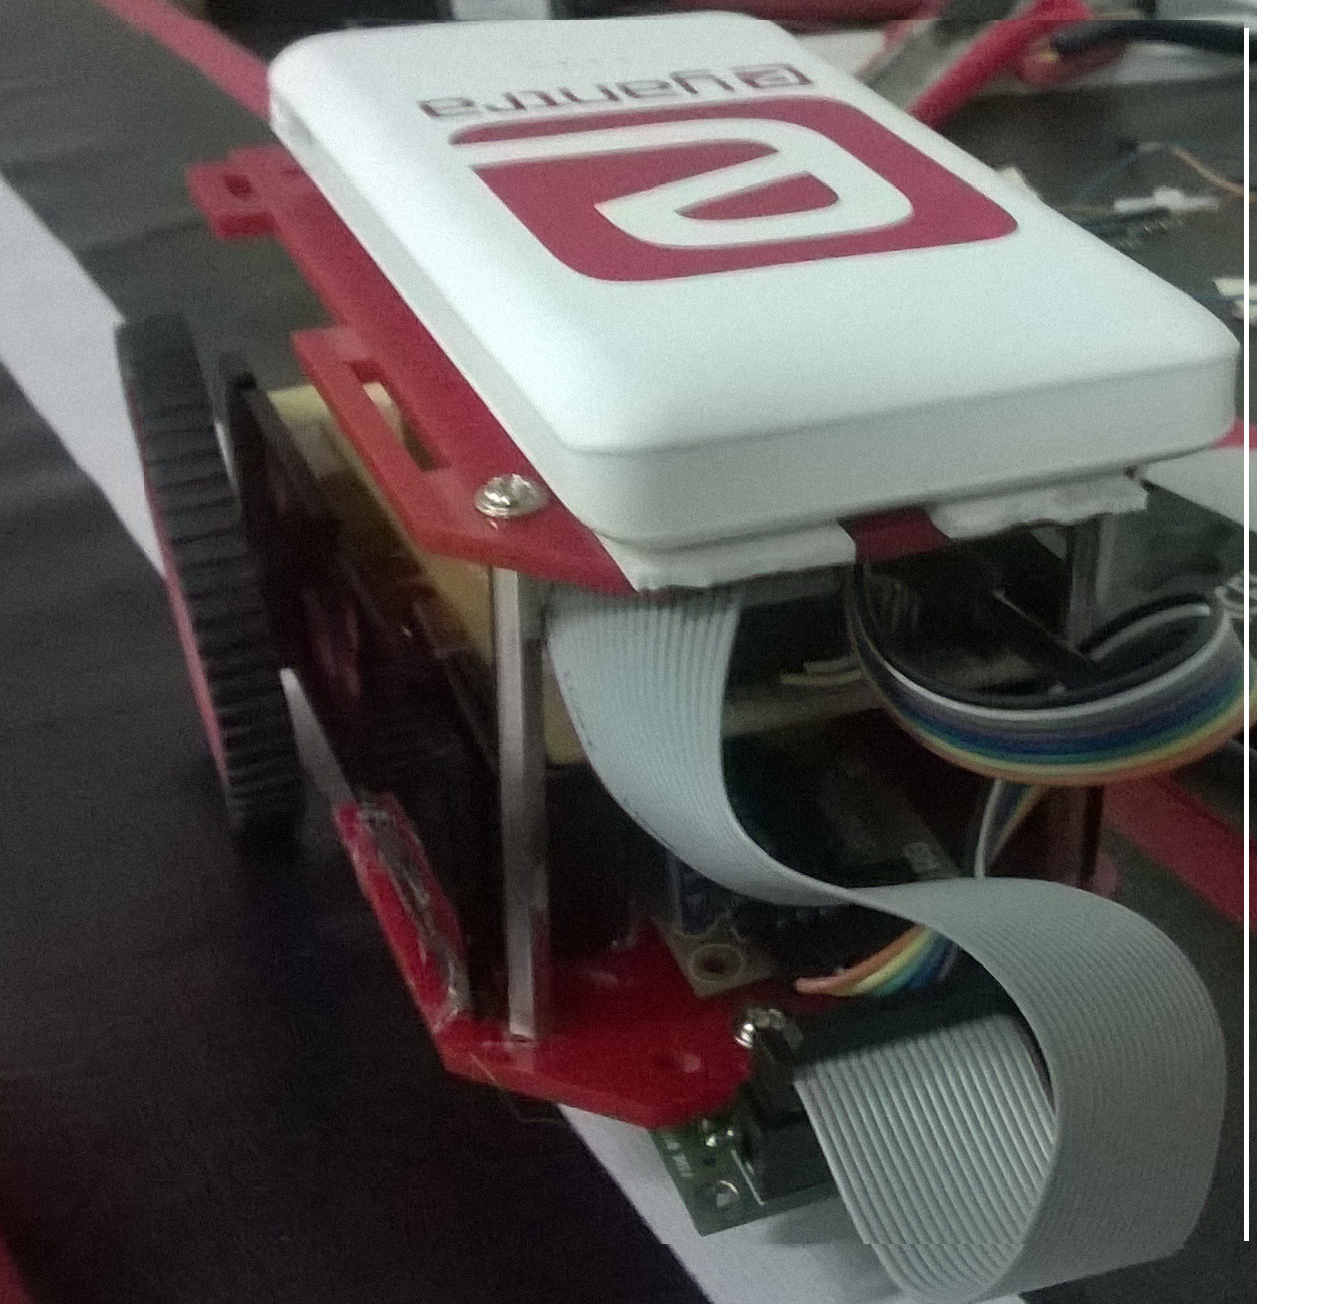
\includegraphics[width=300 px]{img4.png}

\end{enumerate}
\section{Flow Chart:}


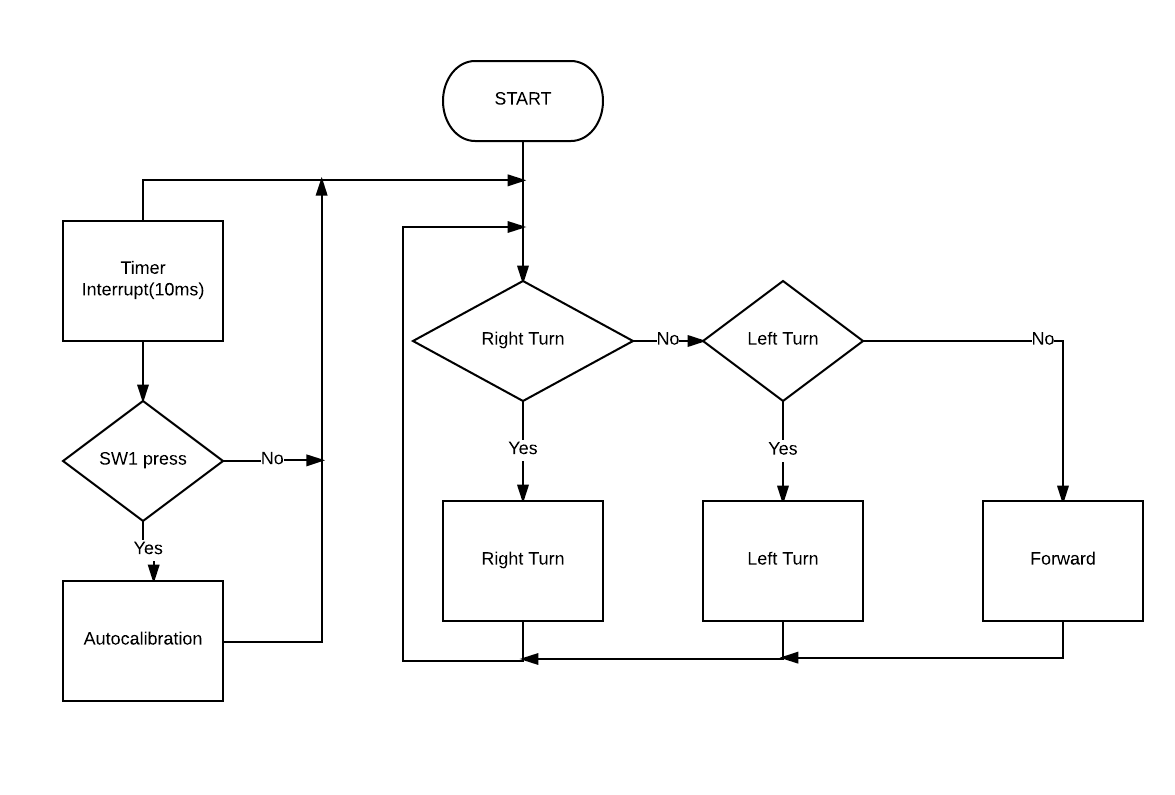
\includegraphics[width=400 px]{flowchart.png}


\section{PROCEDURE}
\begin{enumerate}
\item First intialize eeprom and read the stored value previously written by the code
\item Set the timer which varify the sw1 status at every 10 millisecond and when the swutch is pressed it goes to auto mode.
\item It do the calibration and stores the value in eeprom.
\item Now after it switch from calibration mode,continous to follow on white line.
\item It takes right turn if both sensor on left side have value greater than their threshold and it takes left turn if both sensor on right side are greater than their threshold
\item If above both condition are not satisfeid than it continous forward journey
\end{enumerate}
\section{Challanges}
\begin{enumerate}
\item Assembling the body of robot.
\end{enumerate}
\section{Future plan}
\begin{enumerate}
\item  Sensor such as distance sensor,servo motor,lcd can be interfaced.
\item EEPROM concept can be used to solve the problem such as if robot forgets it's path than it can retraced back.
\end{enumerate}
\section{Code}
\href{https://https://github.com/eYSIP-2016/eYSIP-2016-Around-the-world-of-Embedded-Systems/blob/origin/master/Solutions/Linefollower/linefollower.c}{Github link} for all the codes required for this project.

\section{Demonstration Video}

\href{http://10.129.139.139/videos/Project-Line_Follower.html}{Demo video link} \\
(These videos can be accessed only in IIT Bombay Campus)




%-------------------------------- project 2-------- development board ---
%---------------------Title Page------------------------------------------------


%-------------------------------------------------------------------------------

\chapter[Project Tag]{ Project 2 : ARM CORTEX M4 based Development Board}
\section*{Abstract}
Development board is a development platform based on ARM CORTEX M4 microcontroller. It uses TIVA LaunchPad TM4C123GXL. Other peripherals like push buttons, LEDs, Analog Thumb Joystick, 16X2 LCD, 128X64 GLCD, Xbee, SPI, MPU and Buzzer are connected on the development board. User can start programming these peripherals directly with minimal or no external hardware connections.  

\subsection*{Completion status}
The codes for interfacing push buttons, LEDs, 16X2 LCD, 128X64 GLCD and Analog Thumb Joystick have been completed.

\section{Hardware parts}
\begin{itemize}
  \item TIVA C Series TM4C123G LaunchPad Evaluation Kit\\
  \href{http://www.ti.com/lit/ug/spmu296/spmu296.pdf}{User's Guide}\\
  \href{http://www.ti.com.cn/cn/lit/ds/symlink/tm4c123gh6pm.pdf}{Datasheet}\\
  \href{http://www.ti.com/lit/ug/spmu298a/spmu298a.pdf}{Peripheral Driver Library}
  \item Joystick
  \item 16X2 LCD \\
  \href{http://www.agspecinfo.com/pdfs/J/JHD162A.PDF}{JHD162A Datasheet}\\
  \item 128X64 GLCD\\
  \href{http://www.agspecinfo.com/pdfs/J/JHD12864.PDF}{JHD12864A Datasheet}\\
  \item Schematic of Development Board\\~\\
  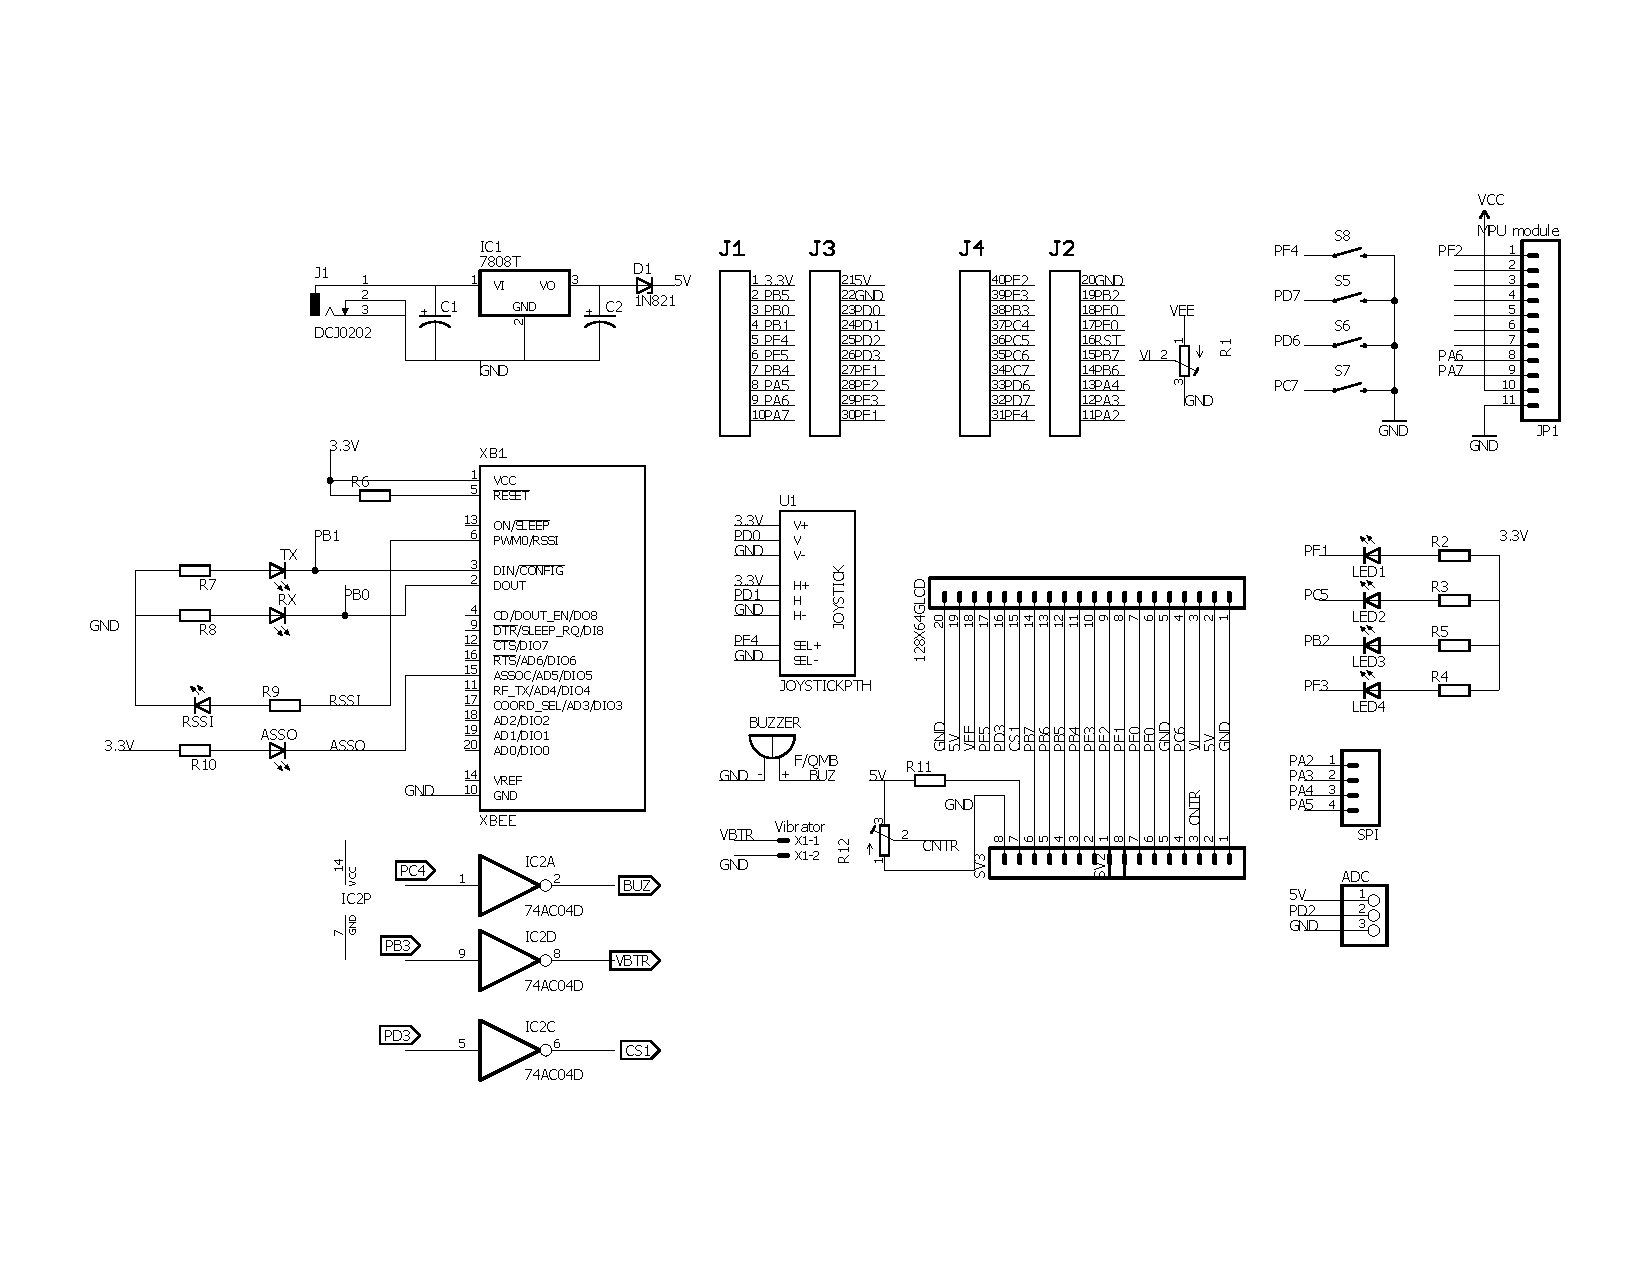
\includegraphics[scale = 0.5]{Gameconsol.pdf}
\end{itemize}

%-------------- s/w used -------------------------

\section{Software used}
\begin{itemize}
  \item Code Composer Studio\\  
  Version 6.1.2 \\
  \href{http://processors.wiki.ti.com/index.php/Download_CCS}{CCS Download Link}\\
  \href{http://processors.wiki.ti.com/index.php/GSG:CCSv6_installation}{CCS Installation steps}
  \item TivaWare\_C\_Series-2.1.2.111\\
  \href{http://www.ti.com/tool/sw-tm4c}{Download Link}
\end{itemize}
%---------------------------------
\newpage
\section{Pin Mapping}



\begin{table}[]
\centering
\begin{tabular}{|c|c|c|}
\hline 
Sr No. & Pin Number & Connected to \\ 
\hline 
1. & PC7 & SW1 \\ 
\hline 
2 & PD6 & SW2 \\ 
\hline 
3. & PD7 & SW3 \\ 
\hline 
4. & PF4 & SW4 \\ 
\hline 
5. & PF1 & LED1 \\ 
\hline 
6. & PC5 & LED2 \\ 
\hline 
7. & PB2 & LED3 \\ 
\hline 
8. & PF3 & LED3 \\ 
\hline 
9. & PD0 & V of Joystick \\ 
\hline 
10. & PD1 & H of Joystick \\ 
\hline 
11. & PE0 to PE3 & D0 to D3 of LCD and GLCD \\ 
\hline 
12. & PB4 to PB7 & D4 to D7 of LCD and GLCD \\ 
\hline 
13. & PC6 & RS for LCD and GLCD \\ 
\hline 
14. & PF0 & Enable of LCD and GLCD \\ 
\hline 
15. & PD3 & CS2 of GLCD \\ 
\hline 
16. & Not PD3 & CS1 of GLCD \\ 
\hline 
17. & PE5 & RST of GLCD \\ 
\hline 
\end{tabular} 
\caption{Pin mapping}
\end{table}

%----------------------------- procedure ------------------
\newpage
\section{Procedure}
\subsection{To program push buttons and LEDs}
\begin{enumerate}
\item Include all the required header files
\begin{lstlisting}
#include <stdint.h>
#include <stdbool.h>
#include "inc/hw_types.h"
#include "inc/hw_memmap.h"
#include "driverlib/sysctl.h"
#include "driverlib/gpio.h"
#include "inc/hw_gpio.h"
#include "driverlib/rom.h"
\end{lstlisting}
\item Enable the System Clock, PORT B, PORT C, PORT D, PORT F. (\textit{Assembly of harware} section gives details about the PORT pins used for different peripherals)
\item Configure the port pins connected to LEDs as output and those connected to push buttons as input.
\item Unlock pin PF0.
\item Read the status of switch and turn on the corresponding LED if switch press is detected.
\item Switch debouncing can also be added if required.
\end{enumerate}

%--------------------- lcd --------------------
\subsection{To program 16X2 LCD}
\begin{enumerate}
\item Include all the necessary header files.
\item Enable System Clock, PORT B, PORT C, PORT E and PORT F.Unlock pin PF0.
\item Refer section \textit{Assembly of hardware} and configure all the required PORT pins as output. (Only LCD write function is implemented hence all pins are output pins)
\item Initialize the LCD in 8 bit mode.
\item Pass the data to be written on LCD to the data lines.
\end{enumerate}


%---------------------- adc -----------------------------
\subsection{Programming Joystick using ADC}
\begin{enumerate}
\item Inlcude all the required header files. Ensure that the following header file is included.
\begin{lstlisting}
#include "driverlib/adc.h"
\end{lstlisting}
\item Enable the System Clock and PORT D.
\item PD0 and PD1 are ADC channels CH7 and CH6 respectively. Configure these pins as ADC input.
\item Configure ADC Sequencer as per requirement. 
\item Enable the ADC.
\item Store the ADC converted data in a variable.
\item This data can be divided by a suitable value. 
\item The final result can be displayed in Watch window, on LCD or on Computer using UART. The movement of Joystick can also be displayed on GLCD.
\end{enumerate}
%-------------------------- glcd -------------------
\subsection{Programming 128X64 GLCD}
\begin{enumerate}
\item To dislay image on GLCD the hex values are calculated. These values are stored in a array in a header file. This header file is included in main program. The array elements can be accessed from the program and written on GLCD data lines.
\item Include all the necessary header files.
\item Enable the System Clock, PORT D, PORT E, PORT F, PORT C.
\item Refer the section \textit{Assembly of hardware} for information regarding connection of PORT pins with GLCD.
\item All the PORT pins are configured as output pins.
\item Initialize and clear the GLCD.
\item To set the GLCD page, page number is logically ORed with 0xB8 and the result is sent to GLCD as GLCD command.
\item To set the GLCD column, column number is logically ORed with 0x40 and the result is sent to GLCD as GLCD command.
\item To display a line on GLCD, select any page number from 0 to 7, select columns from 0 to 127 one after other and write data 0xFF to GLCD.
\end{enumerate}


%---------------------- glcd joystick -------------------------
\subsection{To display movement of Joystick on GLCD}\
\begin{enumerate}
\item Enable and configure System Clock.
\item Configure PORT B, PORT C, PORT D (PD3), PORT E and PORT F as output PORTs.
\item Configure PD0 and PD1 as analog input.(ADC inputs)
\item Configure the ADC.
\item Initialize and clear GLCD.
\item Select a square of 8X8 pixels which will show the position of Joystick on GLCD.
\item To obtain page number the digital value obtained is divided by 512 and for column number the digital value is divided by 32.
\item This value is then sent to GLCD and the movement of Joystick can be observed on GLCD.

\end{enumerate}

\subsection{To control the speed of image on GLCD}
\begin{enumerate}
\item Enable and configure System Clock.
\item Include the header files which contain hex values of images to be displayed.
\item Configure PORT B, PORT C, PORT D (PD3), PORT E and PORT F as output PORTs.
\item Configure PD0 and PD1 as analog input.(ADC inputs)
\item Configure the ADC.
\item Initialize and clear GLCD.
\item Read the analog data from PD0 and PD1. 
\item If the disital data obtained is less than 200 then the delay in between display of two consecutive images is increased.
\item If the disital data obtained is more than 3900 then the delay in between display of two consecutive images is decreased.
\item \href{https://github.com/eYSIP-2016/eYSIP-2016-Around-the-world-of-Embedded-Systems/tree/origin/master/Solutions/development\%20board/controlling\_moving\_images\_on\_glcd}{Github link for code}
\item \href{ http://10.129.139.139/videos/Interfacing_
GLCD_TIVA_Launchpad.html}{GLCD Interfacing Tutorial}
\end{enumerate}

%------------------- code ------------------------
\section{Code}
\href{https://github.com/eYSIP-2016/eYSIP-2016-Around-the-world-of-Embedded-Systems/tree/origin/master/Solutions/development\%20board}{Github link} for all the codes required for this project.

%------------------ demo ------------------------------

\section{Demonstration}
\begin{enumerate}
\item Final Setup Image\\~\\
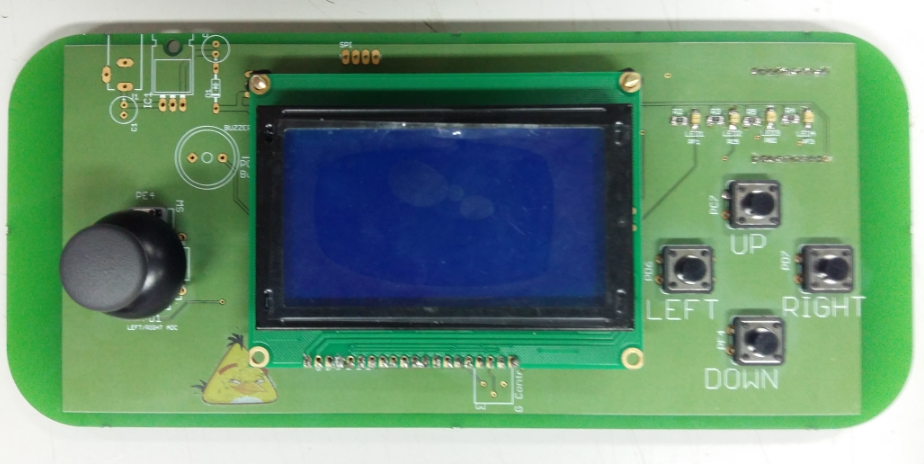
\includegraphics[scale=0.5]{abc.PNG}
\newpage
\item Joystick position displayed on GLCD.\\~\\
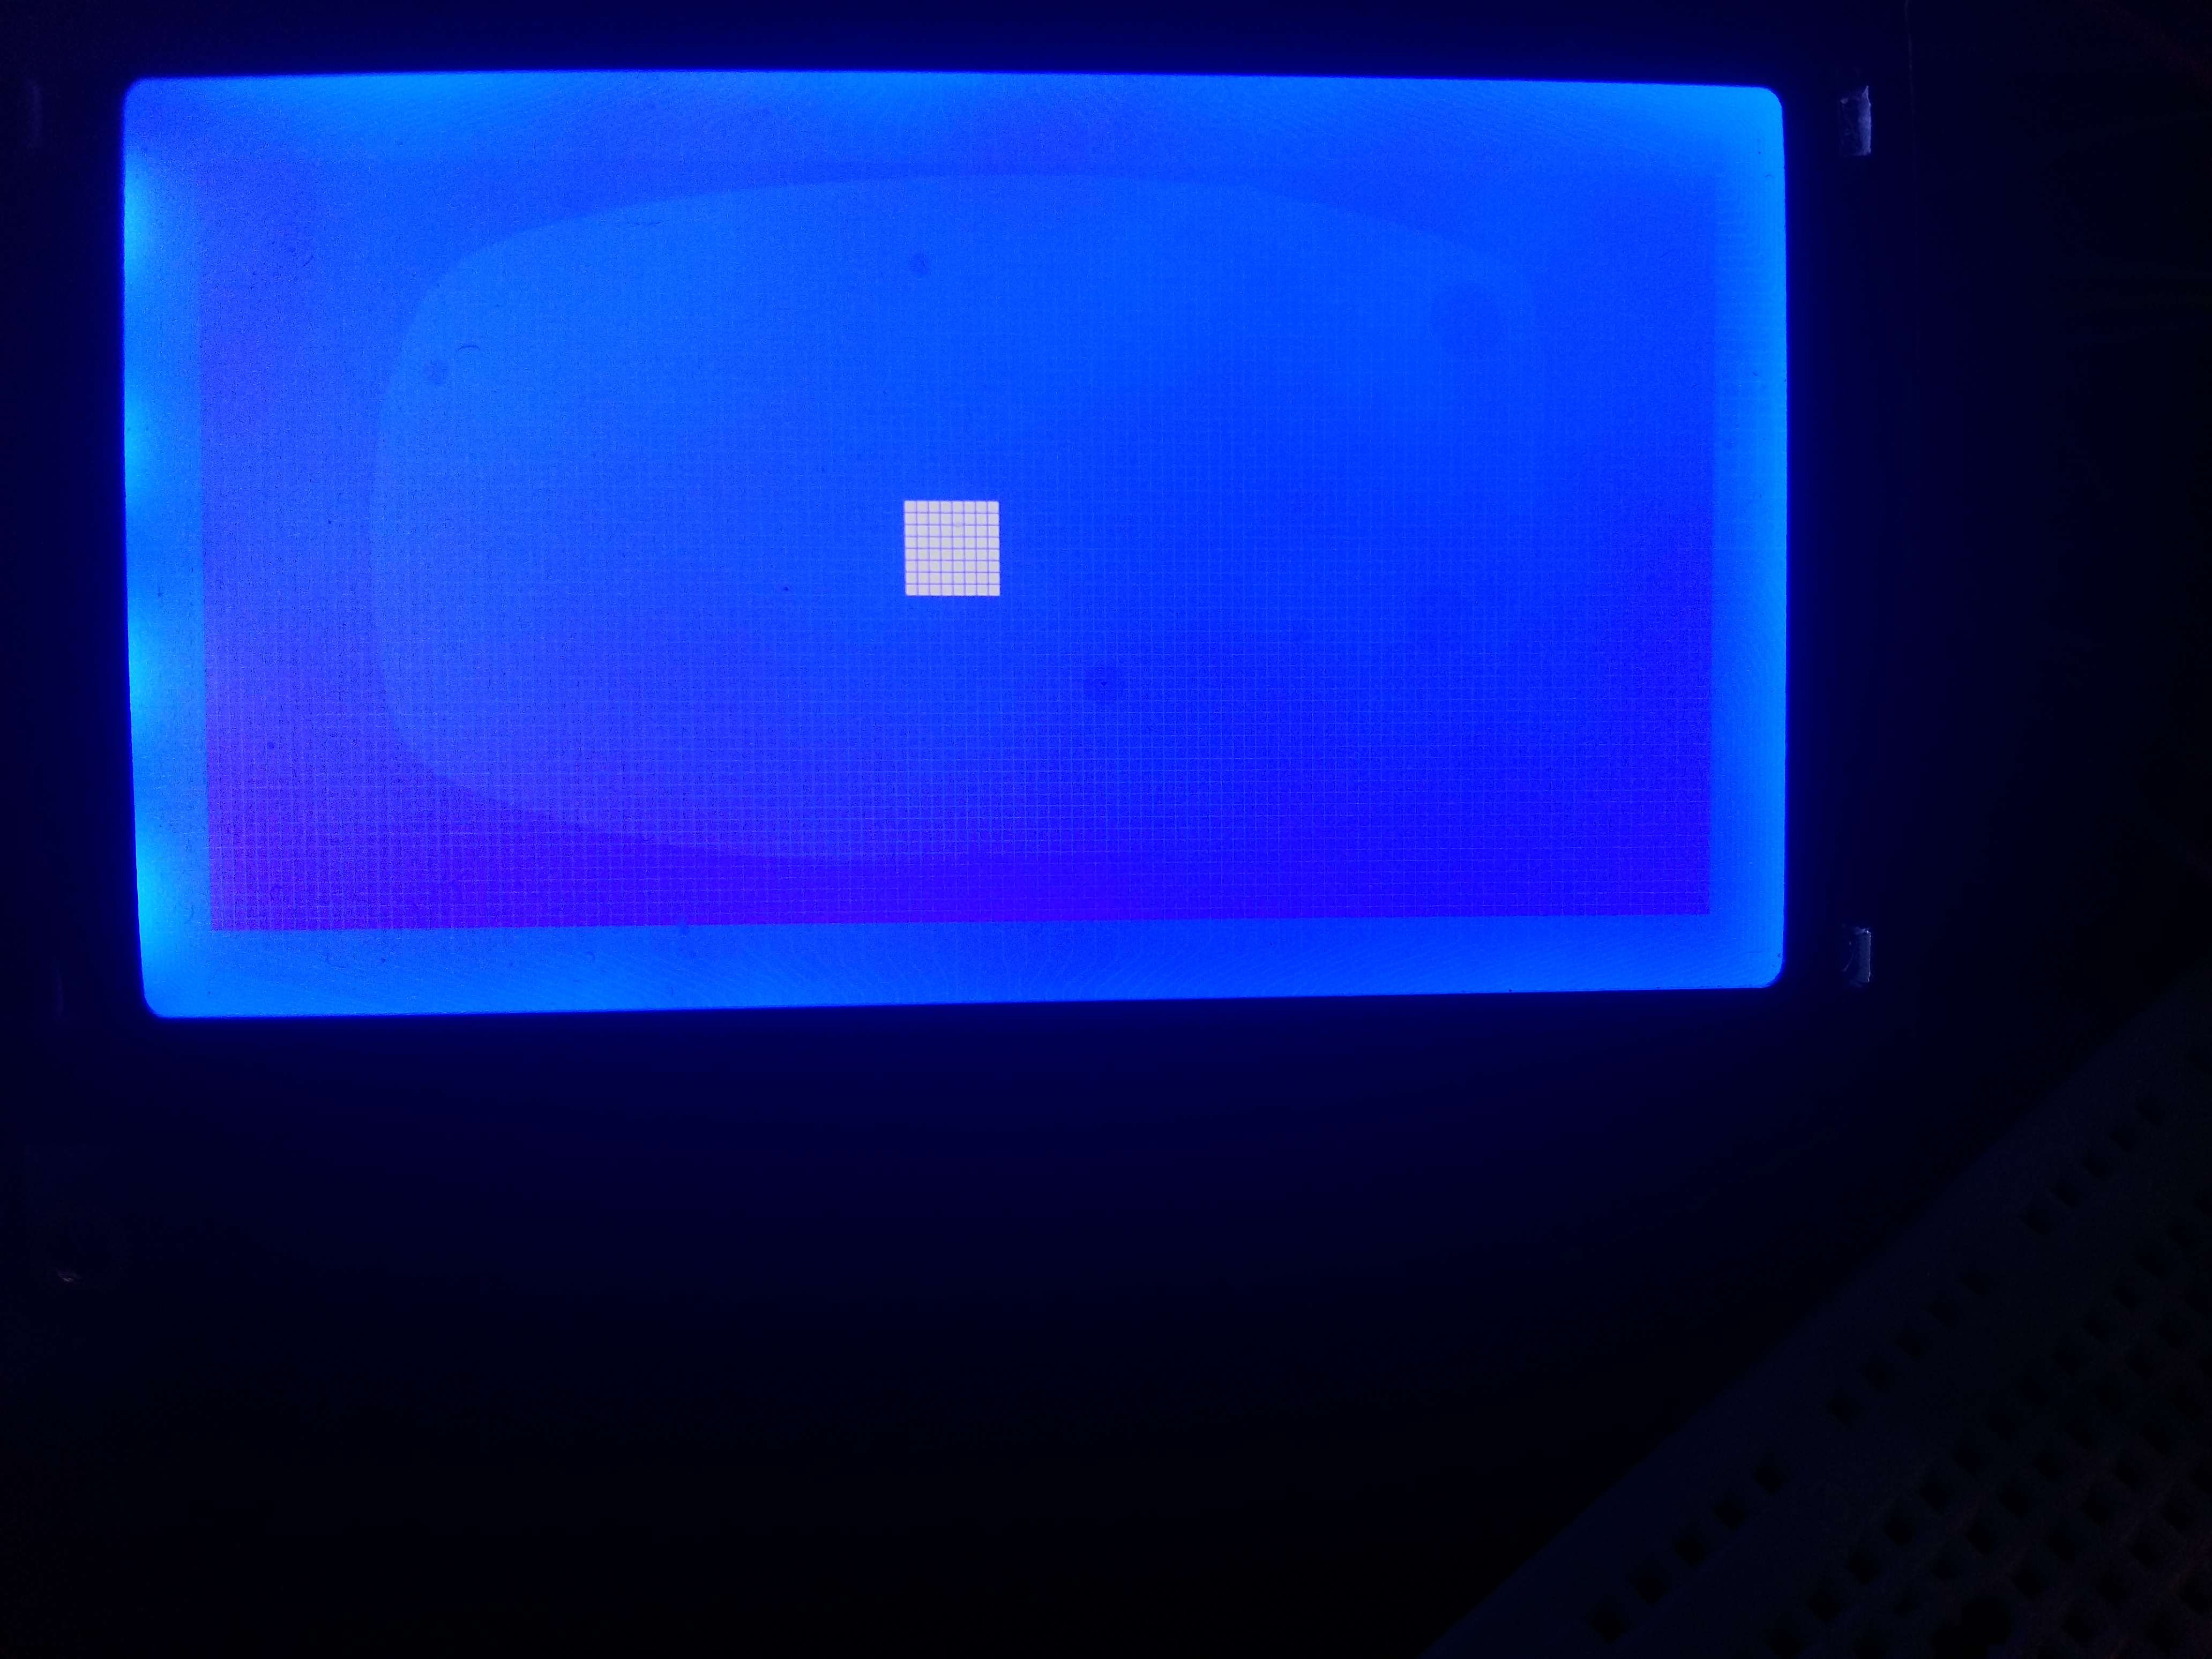
\includegraphics[scale=0.07]{20160708_113016.jpg}
\item Image displayed on GLCD.\\~\\
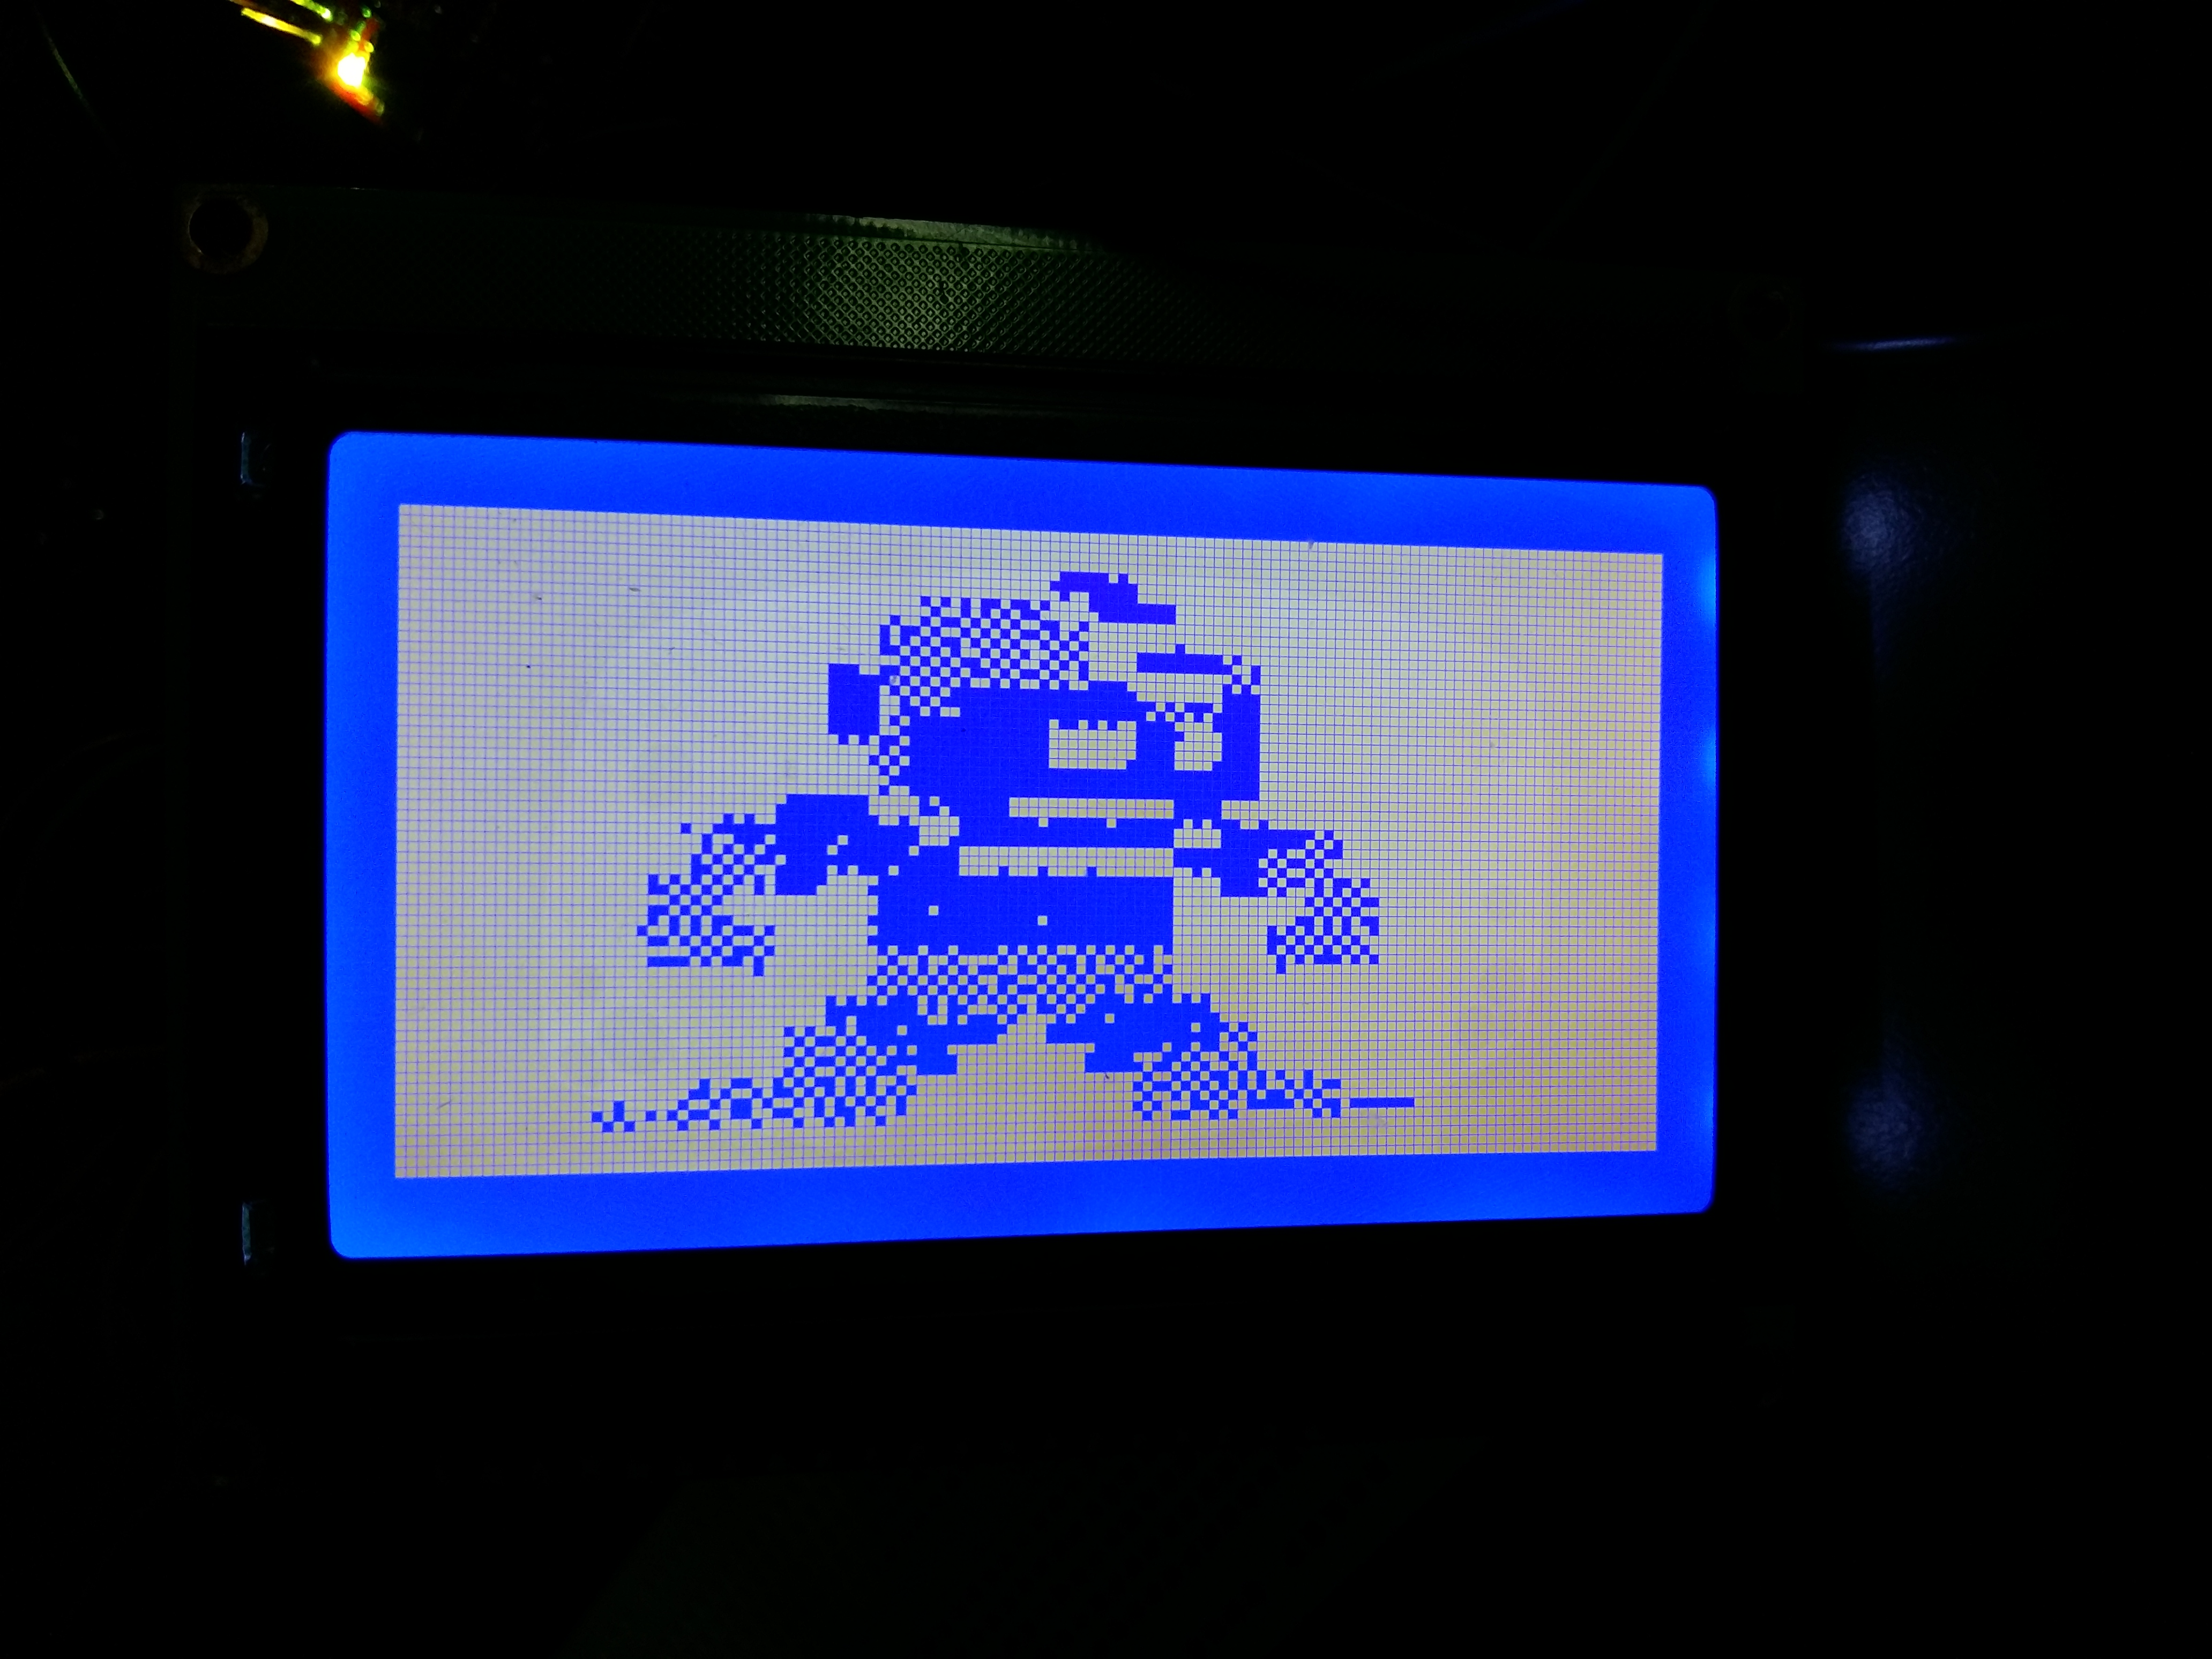
\includegraphics[scale=0.07]{20160706_152740.jpg}
\newpage
\item Moving image on GLCD\\~\\
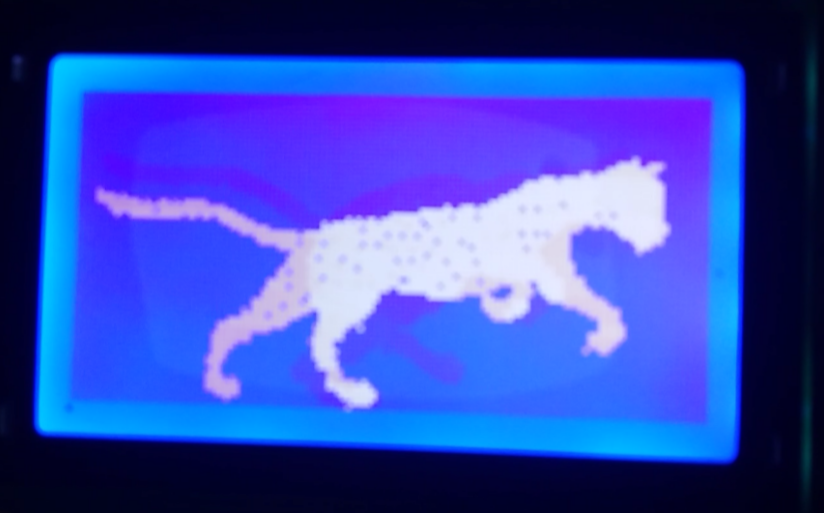
\includegraphics[scale = 0.525]{moving.PNG}

\end{enumerate}


%------------- future work---------------------
\section{Future Work}
A gaming console can be made using Joystick, push button switches and GLCD present on Development Board.


%-------------------- challenges -----------------------
\section{Challenges}
Pin number PB6 and PB7 are internally connected in TIVA Board with PD0 and PD1. PD0 and PD1 are analog input channels of board and PB6, PB7 are data lines D6 and D7 of GLCD. Thus when ADC and GLCD are used simultaneously, expected output is not obtained. \\
For testing the code data lines PB4 to PB7 of GLCD were replaced with PA4 to PA7 and the output was obtained.\\
To use PB4 and PB7 as output data lines and PD0 and PD1 as analog input pins, resistors R9 and R10 on TIVA board were de-soldered.




%---------------------------------------------
\begin{thebibliography}{li}

\bibitem{ 8051 projects}
8051 Projects, {\em LCD Interfacing Tutorial - LCD 4 bit Mode Introduction.}  [Accessed : 8th July 2016] 
\href{http://www.8051projects.net/lcd-interfacing/lcd-4-bit.php}{Website link}

\bibitem{microchip}
Microchip, {\em 16X2 LCD in 4 bit mode.}  [Accessed : 8th July 2016]  
\href{http://www.microchip.com/forums/m656930.aspx}{Website link}

\bibitem{TI}
TI E2E Community, {\em Interfacing TIVA C series to 16X2 LCD.} [Accessed : 8th July 2016] 
\href{https://e2e.ti.com/support/microcontrollers/tiva\_arm/f/908/t/348669}{Website link}

\bibitem{TI}
TI E2E Community,{\em Interfacing TIVA C series to 16X2 LCD.}  [Accessed : 8th July 2016] 
\href{http://www.circuitstoday.com/interfacing-lcd-to-arduino}{Website link}

\bibitem{TI}
TI E2E Community, {\em Connecting Stellaris LaunchPad with 16X2 LCD.}  [Accessed : 8th July 2016] 
\href{https://e2e.ti.com/support/microcontrollers/tiva\_arm/f/908/t/279206}{Website link}

\bibitem{TI}
Circuitstoday,{\em Interfacing LCD to Arduino - Display text and characters on LCD screen using Arduino.}  [Accessed : 8th July 2016] 
\href{https://e2e.ti.com/support/microcontrollers/tiva\_arm/f/908/t/385440}{Website link}


\bibitem{Stack overflow}
Stackoverflow,{\em Plot data points in python using pylab.}  [Accessed : 8th July 2016] 
\href{http://stackoverflow.com/questions/15859534/plot-data-points-in-python-using-pylab}{Website link}

\bibitem{Instructables}
Instructables,{\em Plotting real time data from Arduino using Python}  [Accessed : 8th July 2016] 
\href{http://www.instructables.com/id/Plotting-real-time-data-from-Arduino-using-Python-/}{Website link}


\bibitem{TI}
TI E2E Community,{\em Unlock NMI pin.}  [Accessed : 8th July 2016] 
\href{https://e2e.ti.com/support/microcontrollers/tiva\_arm/f/908/p/298835/1042023}{Website link}



\bibitem{TI}
TI E2E Community,{\em TM4C123G PORT pins locked}  [Accessed : 8th July 2016] 
\href{http://e2e.ti.com/support/microcontrollers/tiva\_arm/f/908/p/398941/1410634}{Website link}


\bibitem{TI}
TI E2E Community,{\em Synthesizing a full 8 bit data port - when seemingly unavailable}  [Accessed : 8th July 2016] 
\href{http://e2e.ti.com/support/microcontrollers/tiva\_arm/f/908/t/279242}{Website link}




\end{thebibliography}
\end{document}

